\documentclass[12pt]{article}
\usepackage{Hoyant_Su}
\usepackage{fancyhdr}
\title{\vspace{-1.4cm}信号时频域分析基础实验}
\author{生物医学工程 \quad 苏浩阳 \quad 20300720002}
\date{2022年09月29日}

\begin{document}

\maketitle
\pagestyle{fancy}
\fancyhead[R]{\songti{20300720002 苏浩阳 \quad 信号时频域分析基础实验}}
\section{实验目的}
\begin{itemize}
\setlength{\itemsep}{0pt}
\setlength{\parsep}{0pt}
\setlength{\parskip}{0pt}
    \item 了解信号的分类:连续—离散,周期—非周期,确定—随机;
    \item 理解傅立叶级数和傅立叶变换分析信号的原理;
    \item 理解信号卷积的时频域关系;
    \item 掌握示波器和频谱仪的基本使用方法;
            掌握ADALM2000(M2K)实验平台的基本使用方法;
            掌握MATLAB信号生成,时频变换的方法。
\end{itemize}

\section{实验原理}
\subsection{MATLAB计算傅里叶变换原理}
工程计算中,傅里叶变换采用数值计算方法,其特点有:1.时间范围有限;2.由于时域的有限性,需要集中频谱能量,防止频谱泄漏;3.时域、频域离散化。

因此,采样类似抽样的方式,对某个频点$f_1+k\Delta f$,将傅里叶变换$X(f_1+k\Delta f)$表示如下:
\begin{center}
     {\setlength\abovedisplayskip{-0.8cm}
     \setlength\belowdisplayskip{-0.2cm}
    \begin{equation}
        \begin{aligned}
            X(f_1+k\Delta f)=\frac{T}{N}\sum^{N-1}_{n=0}x(t_1+n\Delta t)\cdot\mathrm{e}^{-\mathrm{j}2\pi (f_1+k\Delta f)(t_1 +n\Delta t)}          
        \end{aligned}
    \end{equation}
    }
    \label{Fourier}
\end{center}



式\ref{Fourier}中,$N$为抽样点数,$\Delta t$为时域间隔,T为有限时域时长。

采用频域间隔$\Delta f$,在区间$[f_1,f_2]$上通过式\ref{Fourier}计算,即得到频域离散化的傅里叶变换。

\subsection{计算傅里叶变换的四种方法}
MATLAB计算傅里叶变换可采用1.解析表达式法;2.双重循环法;3.向量计算法及4.矩阵计算法。

对解析表达式法,采用fourier\(\)直接计算,但要求括号内只能为解析表达式的确定形式。

双重循环法模拟对时域、频域采样,采用式\ref{Fourier}计算傅里叶变换,其中,外层for循环为频域采样、内层for循环为时域采样。

向量计算法将单一频点的离散时间傅里叶变换表达式改写如下:

\begin{center}
     {\setlength\abovedisplayskip{-0.8cm}
       \setlength\belowdisplayskip{-0.8cm}
    \begin{equation}
        \begin{aligned}
          X(f_1+k\Delta f)=\frac{T}{N}
\begin{bmatrix}
 \mathrm{e}^{-\mathrm{j}2\pi (f_1+k\Delta f)t_1} &\mathrm{e}^{-\mathrm{j}2\pi (f_1+k\Delta f)(t_1 +\Delta t)}  & ... &\mathrm{e}^{-\mathrm{j}2\pi (f_1+k\Delta f)(t_2 -\Delta t)}
  \end{bmatrix}
 \begin{bmatrix}
  x(t_1)\\
  x(t_1+\Delta t)\\
  ...\\
  x(t_2-\Delta t)
\end{bmatrix}  
        \end{aligned}
    \end{equation}
    }
    \label{Fourier_vector}
\end{center}


矩阵计算法构造\mathbf{F}矩阵,\mathbf{F}矩阵为行为频率采样点数、列为时间采样点数的矩阵。有:
\begin{center}
     {\setlength\abovedisplayskip{-0.8cm}
      \setlength\belowdisplayskip{-0.8cm}
    \begin{equation}
        \begin{aligned}
        \mathbf{X}=\frac{T}{N}\mathbf{F}\mathbf{x}
        \end{aligned}
    \end{equation}
    }
    \label{matrix_Fourier}
\end{center}

\subsection{MATLAB计算卷积原理}
基于MALTAB的卷积近似计算式为
\begin{center}
     {\setlength\abovedisplayskip{-0.6cm}
       \setlength\belowdisplayskip{-0.8cm}
\begin{equation}
    \begin{aligned}
y(nT)=T\sum_{m=-\infty}^{\infty}x(mT)h(nT-mT)
    \end{aligned}
\end{equation}    
}
\label{conv}
\end{center}


%%%%%%%%%%%%%%%%%%%%%%%%%%%%%%%%%%%%%%%%%%%%%%这里还缺一个相关的表达式%%%%%%%%%%%%


\subsection{信号加窗原理}
\subsubsection{窗函数的作用}
从工程角度,对无限长信号,实际采集到的信号是有限的。采用FFT算法时,FFT将信号在时域及频域上构成环形结构,即将采集到的有限信号前后相连。若采集信号未构成完整周期,即FFT变换相连后信号值发生突变,则使得采样处理后的信号与原信号不一致,且突变的片段在FFT处理后形成高频成分,进而产生频谱泄漏。

为减少频谱泄漏,需在已采集的有限信号上加窗,窗函数可减少FFT处理后,信号不连续部分的突变,使之尽可能呈现连续波形,进而减少频谱泄漏。

\subsubsection{窗函数的类型}
实验中采用的窗函数有矩形窗、汉宁窗、汉明窗等。
\begin{table}[H]
		\setlength{\abovecaptionskip}{0cm} 
		\setlength{\belowcaptionskip}{0.2cm}
    \centering
        \caption{窗的类型及软件表示}
    \begin{tabular}{clll}
    \toprule[1.2pt]
        窗的类型 & MATLAB & SCOPY & 时域表达式\\
        \midrule
       矩形窗  & boxcar\(\)&Rectangular & $\omega(t)=1, 0\le t\le N-1 $\\
        汉宁窗 & hann\(\)& Hann & $\omega(t)=\frac{1}{2}\cdot (1-\cos{\frac{2\pi (t-1)}{N-1}}), 0\le t\le N-1 $\\
        汉明窗 &hamming\(\) & Hamming & $\omega(t)=0.54 - 0.46\cos{\frac{2\pi t}{N-1}}, 0\le t\le N-1 $\\
         \bottomrule[1.2pt]
    \end{tabular}
    \label{window}
\end{table}




\section{实验内容及实验分析}
\setcounter{subsection}{-1}
\subsection{预习实验:傅里叶变换的数值计算}
\textbf{实验要求}:1.用双重循环法计算傅里叶变换的函数;2.用向量乘法或用矩阵乘法计算傅里叶变换的函数(二选一)。测量不同函数在不同数据量下的计算时间。

\textbf{实验代码编写及分析}:

1.用\textbf{双重循环法}实现傅里叶变换:根据式\ref{Fourier},对每个频点,在时域上采样,因此对时域内循环;在频域上采样,从而将频点扩展到频谱,因此对频域外循环。代码如下\footnote{只给出最核心部分代码,省略输入信号的参数选择及绘图部分。}:
\begin{lstlisting}
    %%%%%%此处省略输入信号的选择及参数的设定%%%%%%%%%
    f_t = 1; t_t = 1; % 频域采样下标及时域采样下标
    total = 0; 
    tic % 运行时间测量
    for f = f1:df:f2
        for t=t1:dt:t2
            num=T/N*(exp(-1j*2*pi*f*t)) * y(t_t) * w(t_t);%此处w为选定的窗函数
            total = total + num;
            t_t = t_t + 1;
        end
        F(f_t) = abs(total); % F为频域函数
        f_t = f_t + 1;
        total = 0;
        t_tail = 1;
    end
    toc % 运行时间测量
    %%%%%%%%%%%此处省略绘图部分代码%%%%%%%%%%%%%%%%
\end{lstlisting}

2.用\textbf{用向量乘法}实现傅里叶变换:根据式\ref{Fourier_vector},对每个频点,其对应频域函数可用时域上一组行向量与一组列向量的乘积表示,因此向量乘法只需频域上一组循环,省略了时域内循环。代码如下:
\begin{lstlisting}
    x1 = x .* hm';   %时间信号x过窗,变为x1
    for k=f1:df:f2
        F(k)=abs(T / N * exp(-2j * pi * k * t) * x1'); 
        % t为一行向量,exp(-2j * pi * k * t)组成向量乘积法的行向量,x1'组成向量乘积法的列向量
    end
\end{lstlisting}

\textbf{双重循环法及向量乘法计算时间的测量:}
采样正弦信号$x(t)=\sin (2\pi\cdot 1000 \cdot t)$进行测试,窗长$T$固定为0.01,以汉宁窗截断,通过改变时域采样间隔的方式改变数据量,用MALTAB,tic-toc测量结果如下:
\begin{table}[H]
		\setlength{\abovecaptionskip}{0cm} 
		\setlength{\belowcaptionskip}{0.2cm}
    \centering
     \caption{不同函数在不同数据量下的计算时间}
    \begin{tabular}{lrrrr}
    \toprule[1.5pt]
    \midrule
       时域步长  & $0.1\mu s$ & $1\mu s$ & $10\mu s$ & $100\mu s$\\
         \midrule
       双重循环法 & 104.99 s & 14.697 s & 1.8910 s & 0.20866 s\\
        向量乘法  & 10.661 s & 2.1875 s & 0.24730 s & 0.04270 s\\
         \bottomrule[1.5pt]
    \end{tabular}
    \label{runtime}
\end{table}

横向比较表\ref{runtime}的数据,可知随着数据量的增大,运行时间与之呈正相关,在双重循环法中,这种正相关性更明显,表现为数据量增大时,运行时间显著上升,数据量减小时,运行时间也迅速下降;而向量乘积法中,当数据量增大时,运行时间不会显著上升,数据量减小时,运行时间也不会显著下降。这可以解释为,对双重循环法,数据量的增大与内存分配的次数是成正比的;而对向量乘法,内存的分配是连续的,不与数据量完全成正比例,只保留了正相关性。

纵向比较表\ref{runtime}的数据,同一数据量下,向量乘法运行时间均远小于双重循环法运行时间,这可以解释为MATLAB的向量化表达在运行开始时就建立了连续的内存空间,而双重循环法在每次循环调用时均重新分配内存,导致运行时间增长;另一方面,MATLAB的高性能数学库也加快了向量乘法、矩阵乘法的运行速度。从时间复杂度上:双重循环的复杂度为$O(n^2)$,而向量乘法只需对每个频点采样,复杂度为$O(n)$,因此向量乘法运行时间短。




\subsection{实验一:单音信号,2kHz正弦波}
\subsubsection{示波器测量单音正弦信号}
\textbf{实验要求a}:用波形发生器产生一个2kHz正弦波,用示波器观察其时域波形并记录;用FFT功能观察频谱并记录;采用几种窗函数形式记录频谱,并分析其变化原因。

\textbf{实验过程}:将示波器输入电缆连接信号发生器,信号发生器设为2kHz,峰峰值为5V的正弦信号,待示波器波形稳定后,旋转示波器水平旋钮,使屏幕上显示约七个周期的正弦波形。按下Math模式,按下FFT功能,按下水平按键,并将精度调至5.00kHz/div。此时观察到红色单峰谱线,按下Menu off,并利用光标法测得其频点约2.0000kHz。

实验测量结果如下:
\begin{figure}[H]
    \centering
    
    \subfigure[subfigure 1-1][汉明窗]{
        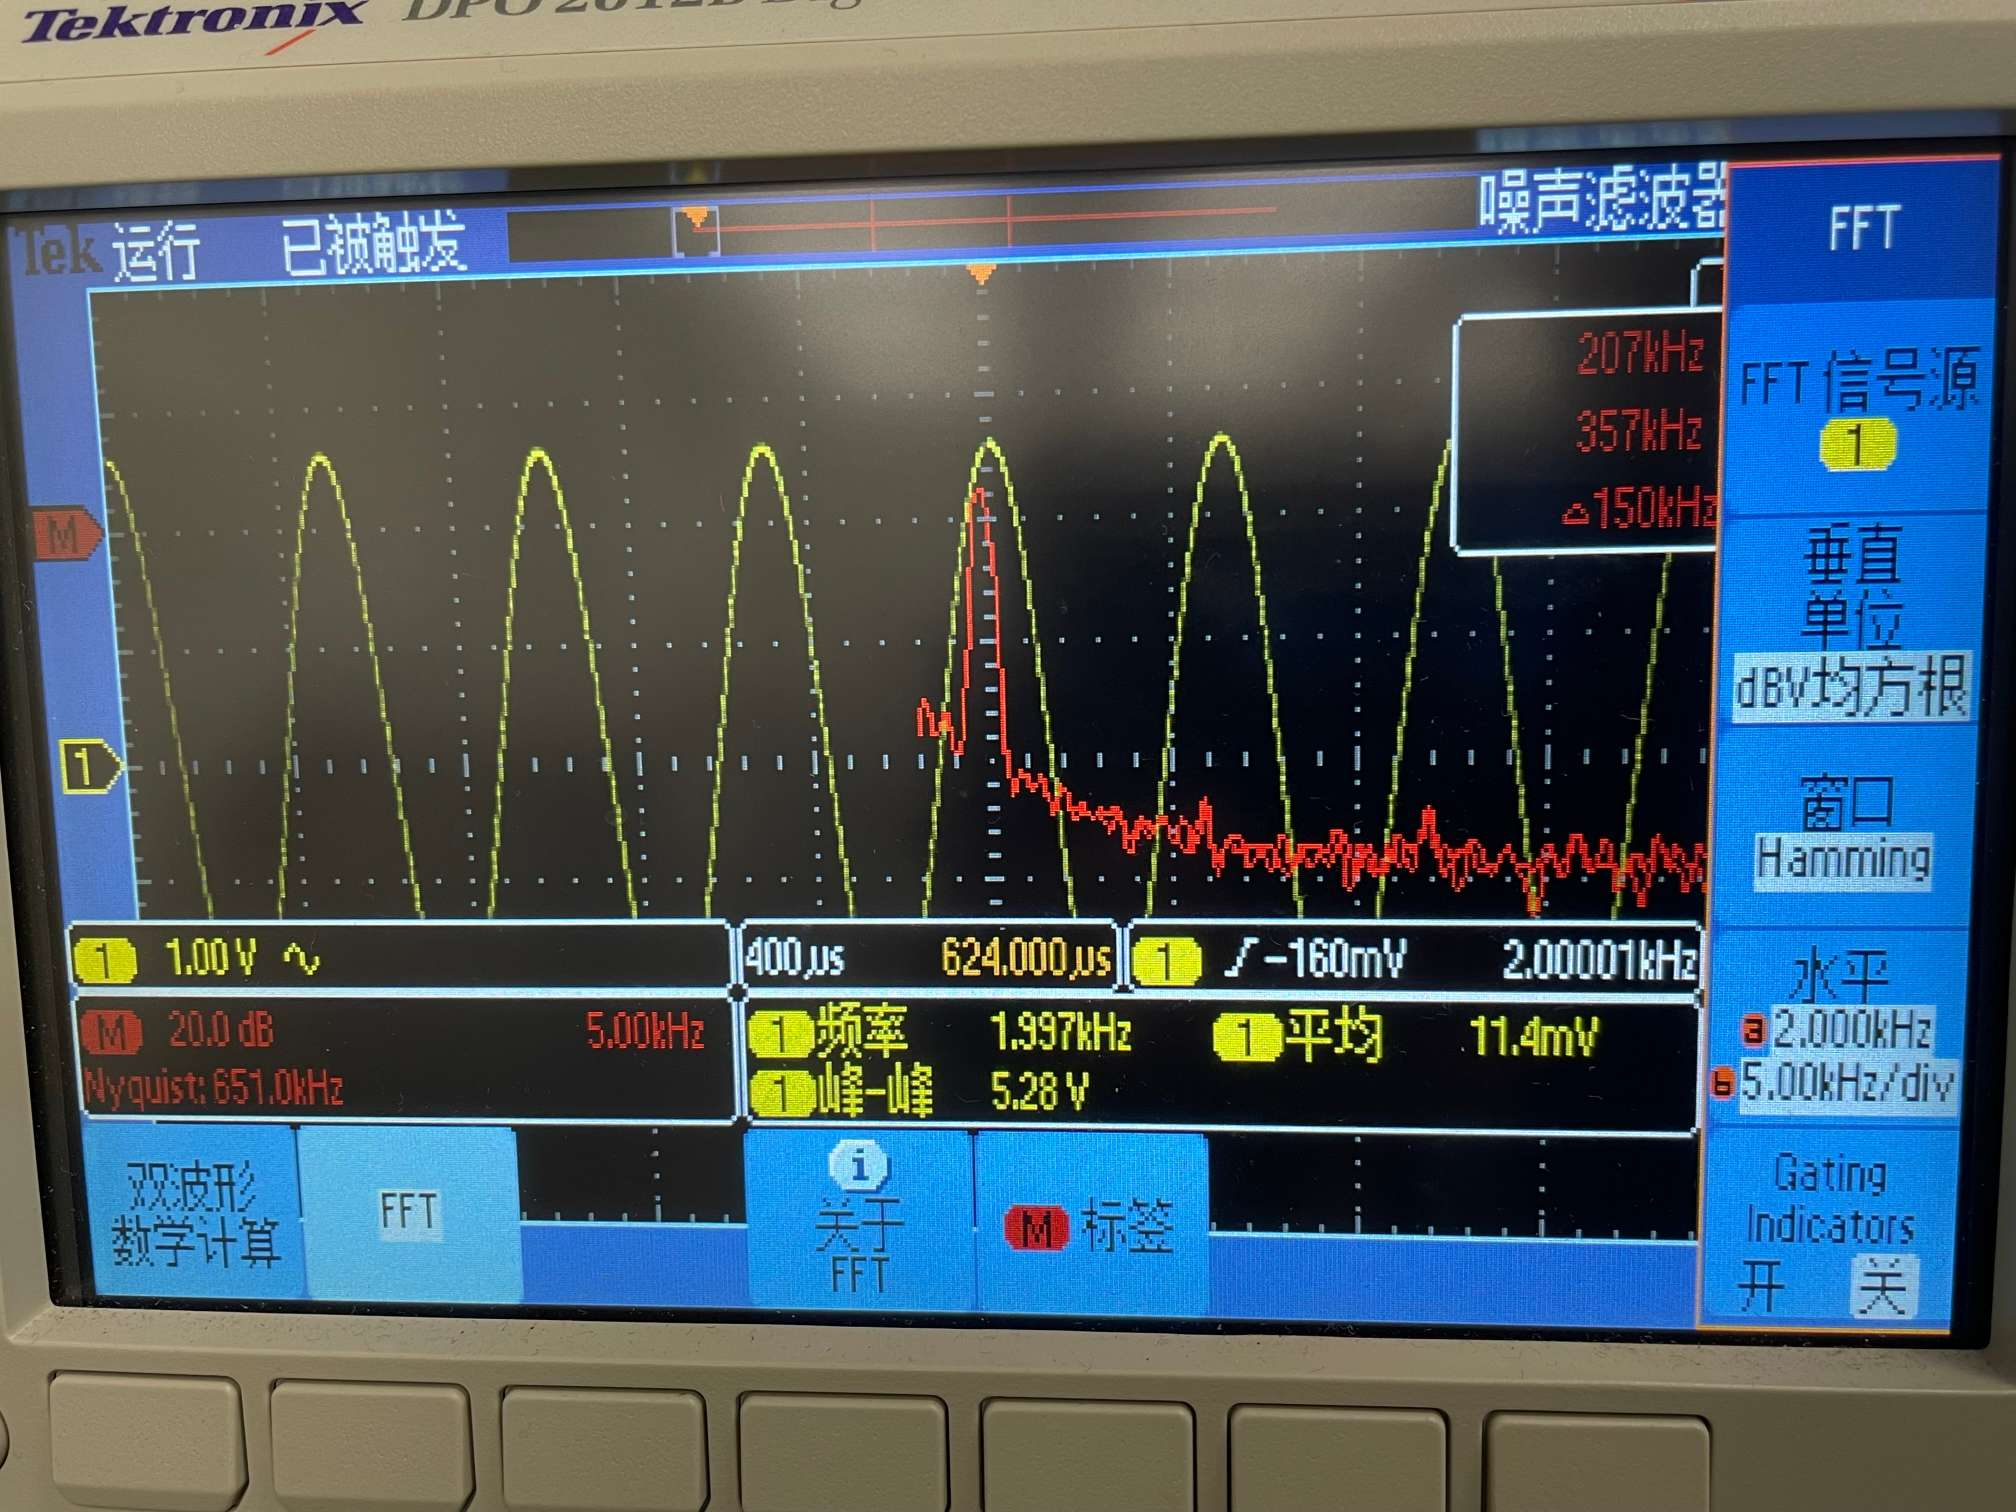
\includegraphics[width=0.3\textwidth]{hamming_sine_osc.jpg}
    }
     \hspace{0.005\linewidth}
      \subfigure[subfigure 1-2][汉宁窗]{
        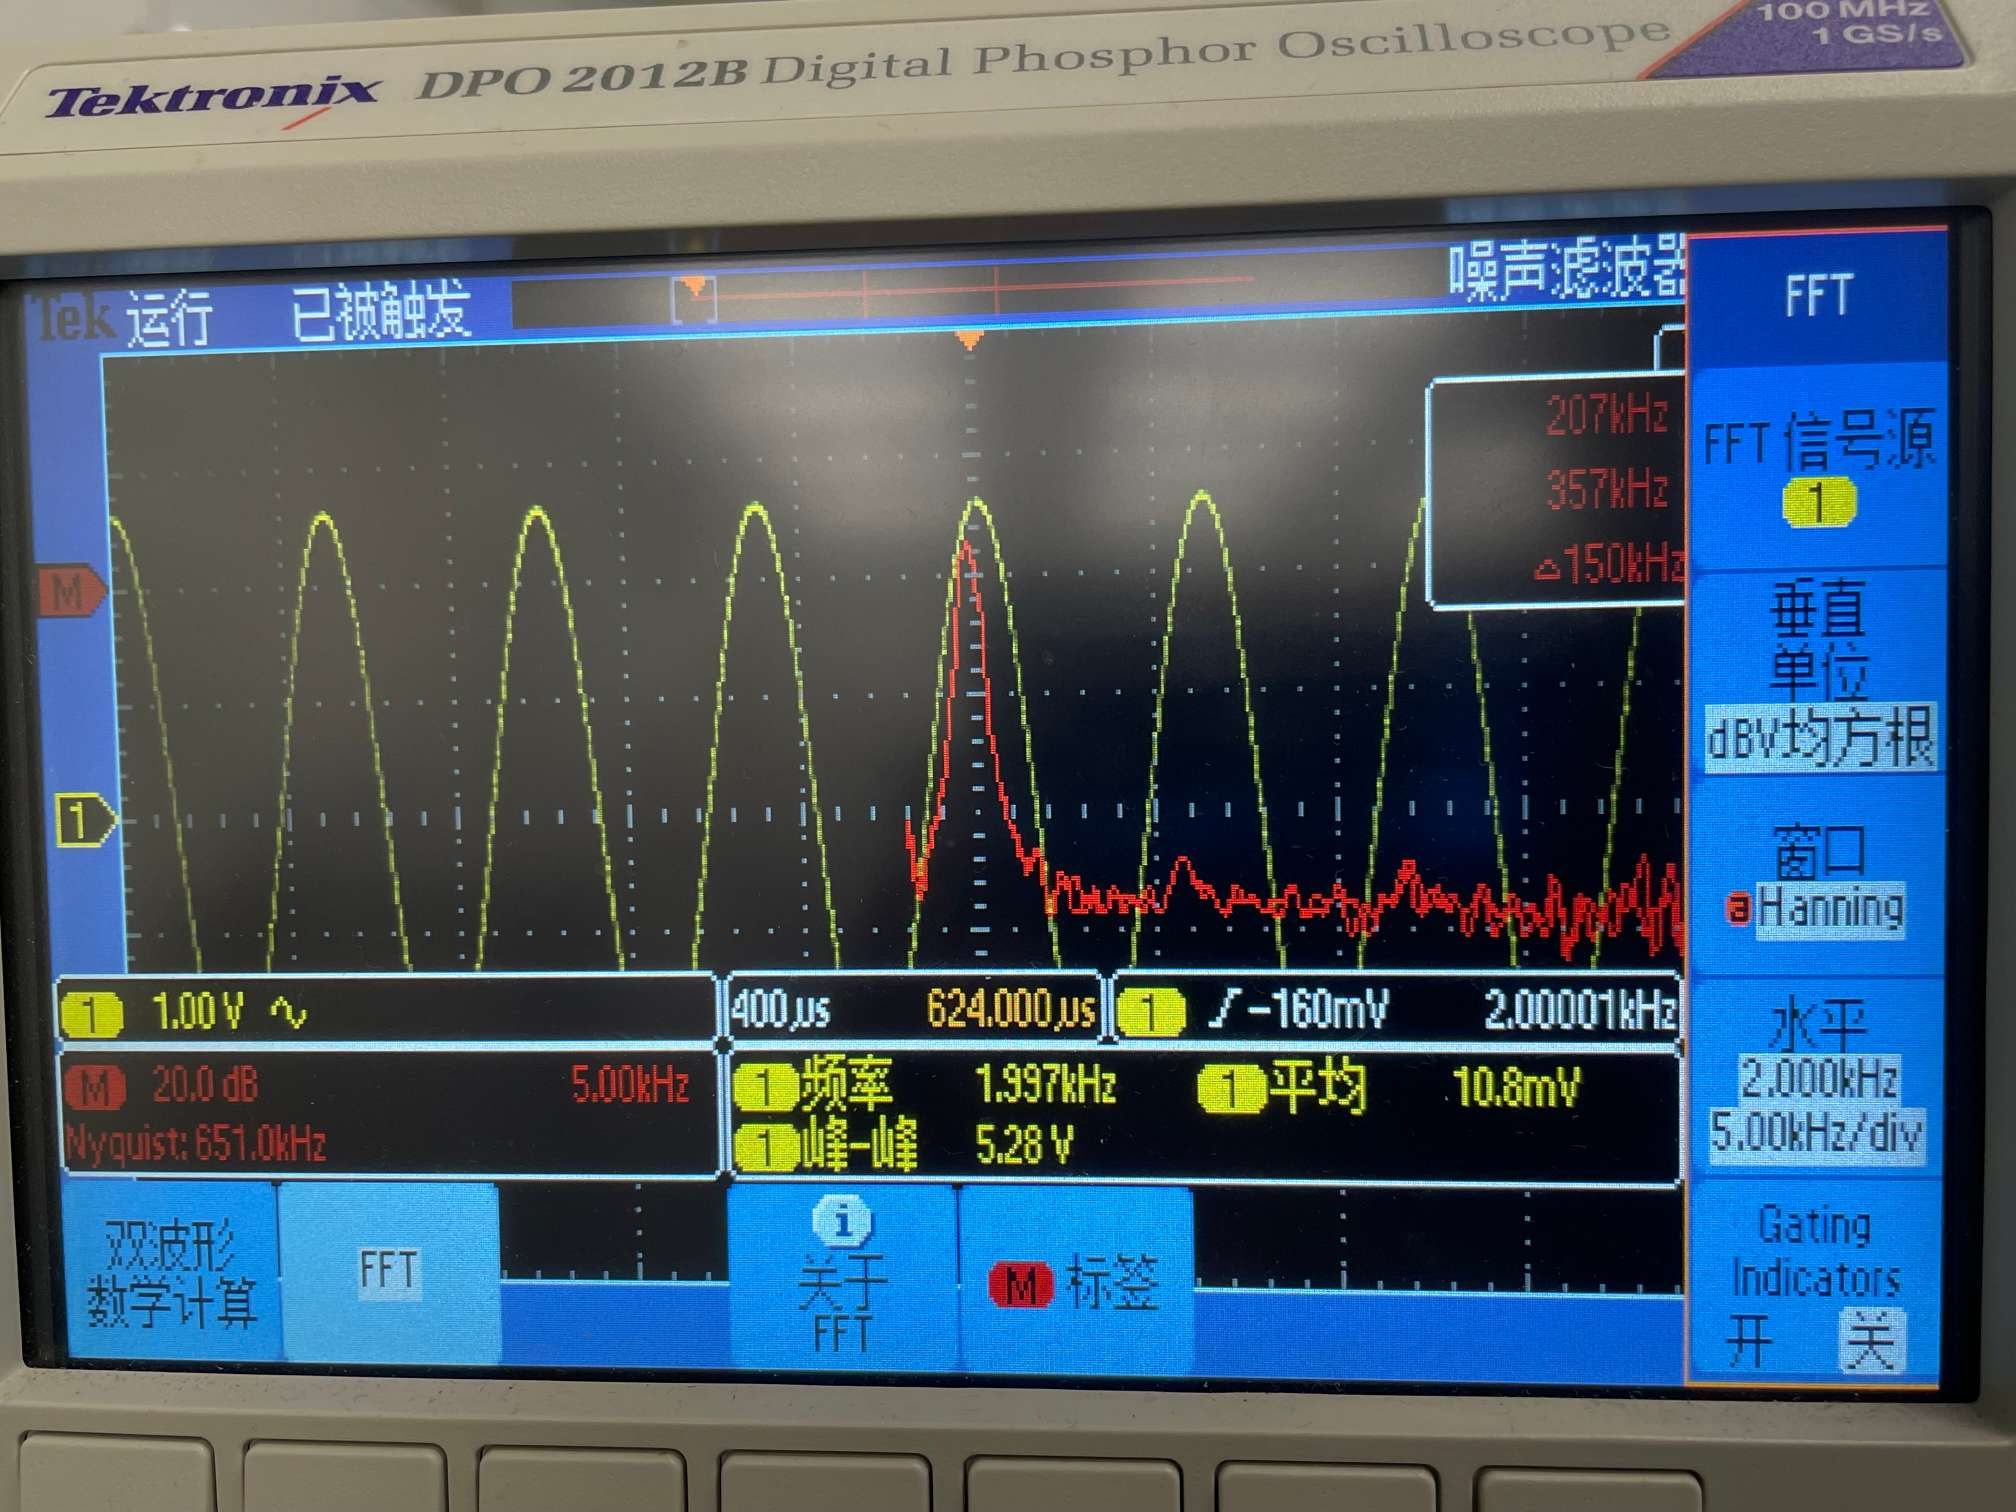
\includegraphics[width=0.3\textwidth]{hanning_sine_osc.jpg}
    }
         \hspace{0.005\linewidth}
      \subfigure[subfigure 1-3][矩形窗]{
        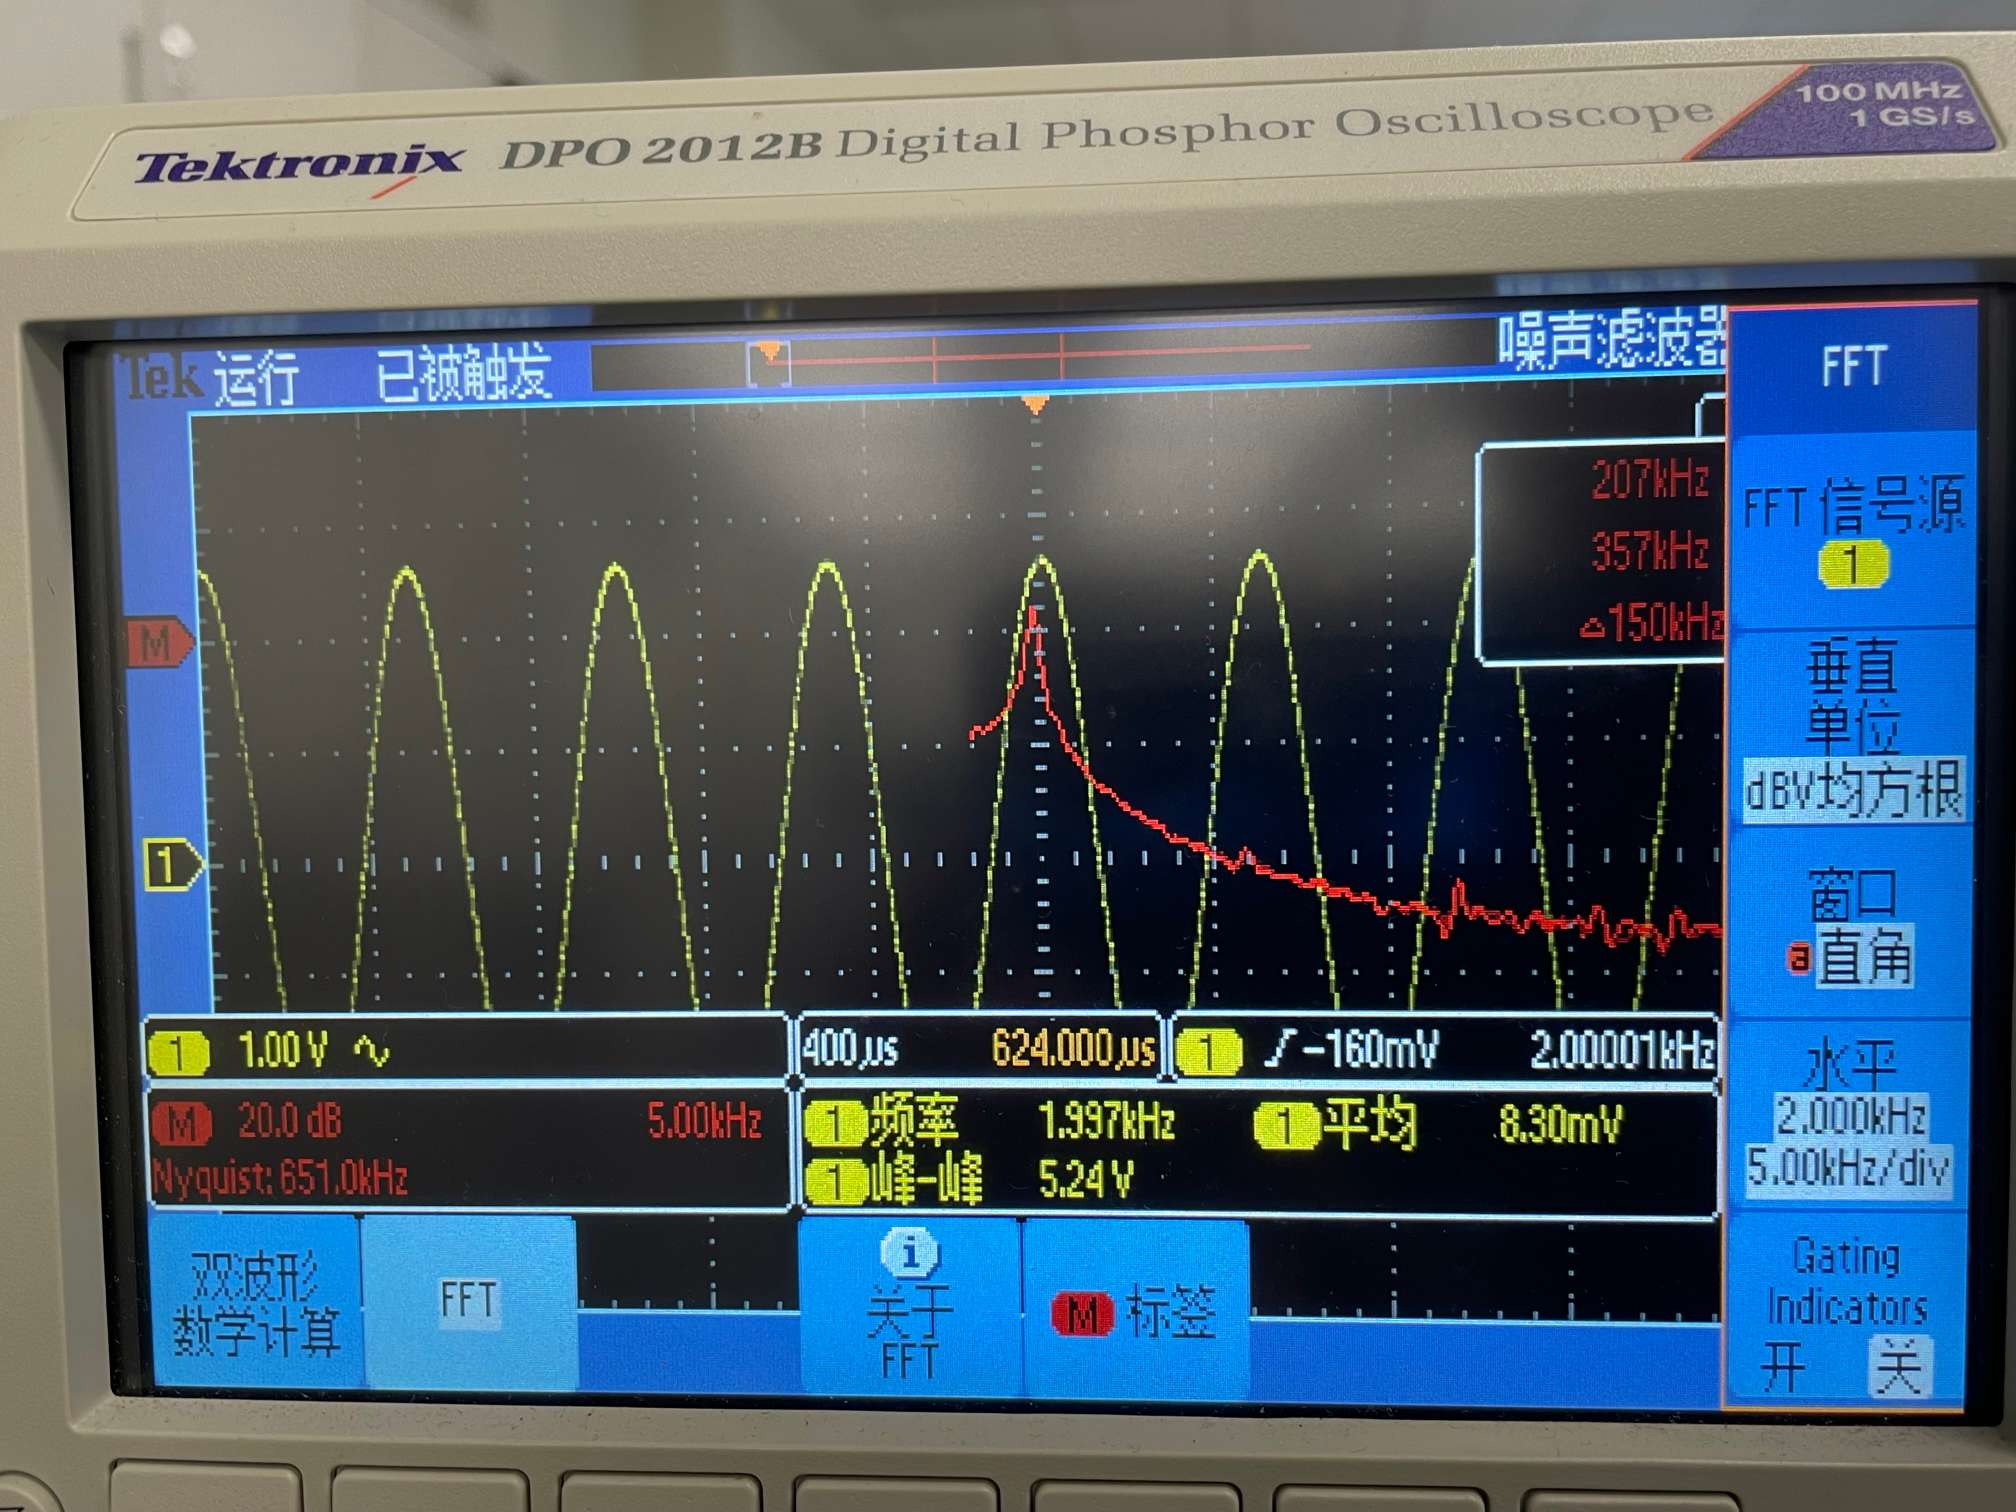
\includegraphics[width=0.3\textwidth]{rect_sine_osc.jpg}
    }
    \caption{示波器显示正弦单音信号时频域波形}
  \label{示波器1a}
\end{figure}

调整波形垂直旋钮,并将光标移至谱线峰值处,测量结果如下各子图右上角所示:
\begin{figure}[H]
    \centering
    
    \subfigure[subfigure 1-1][汉明窗频谱测量]{
        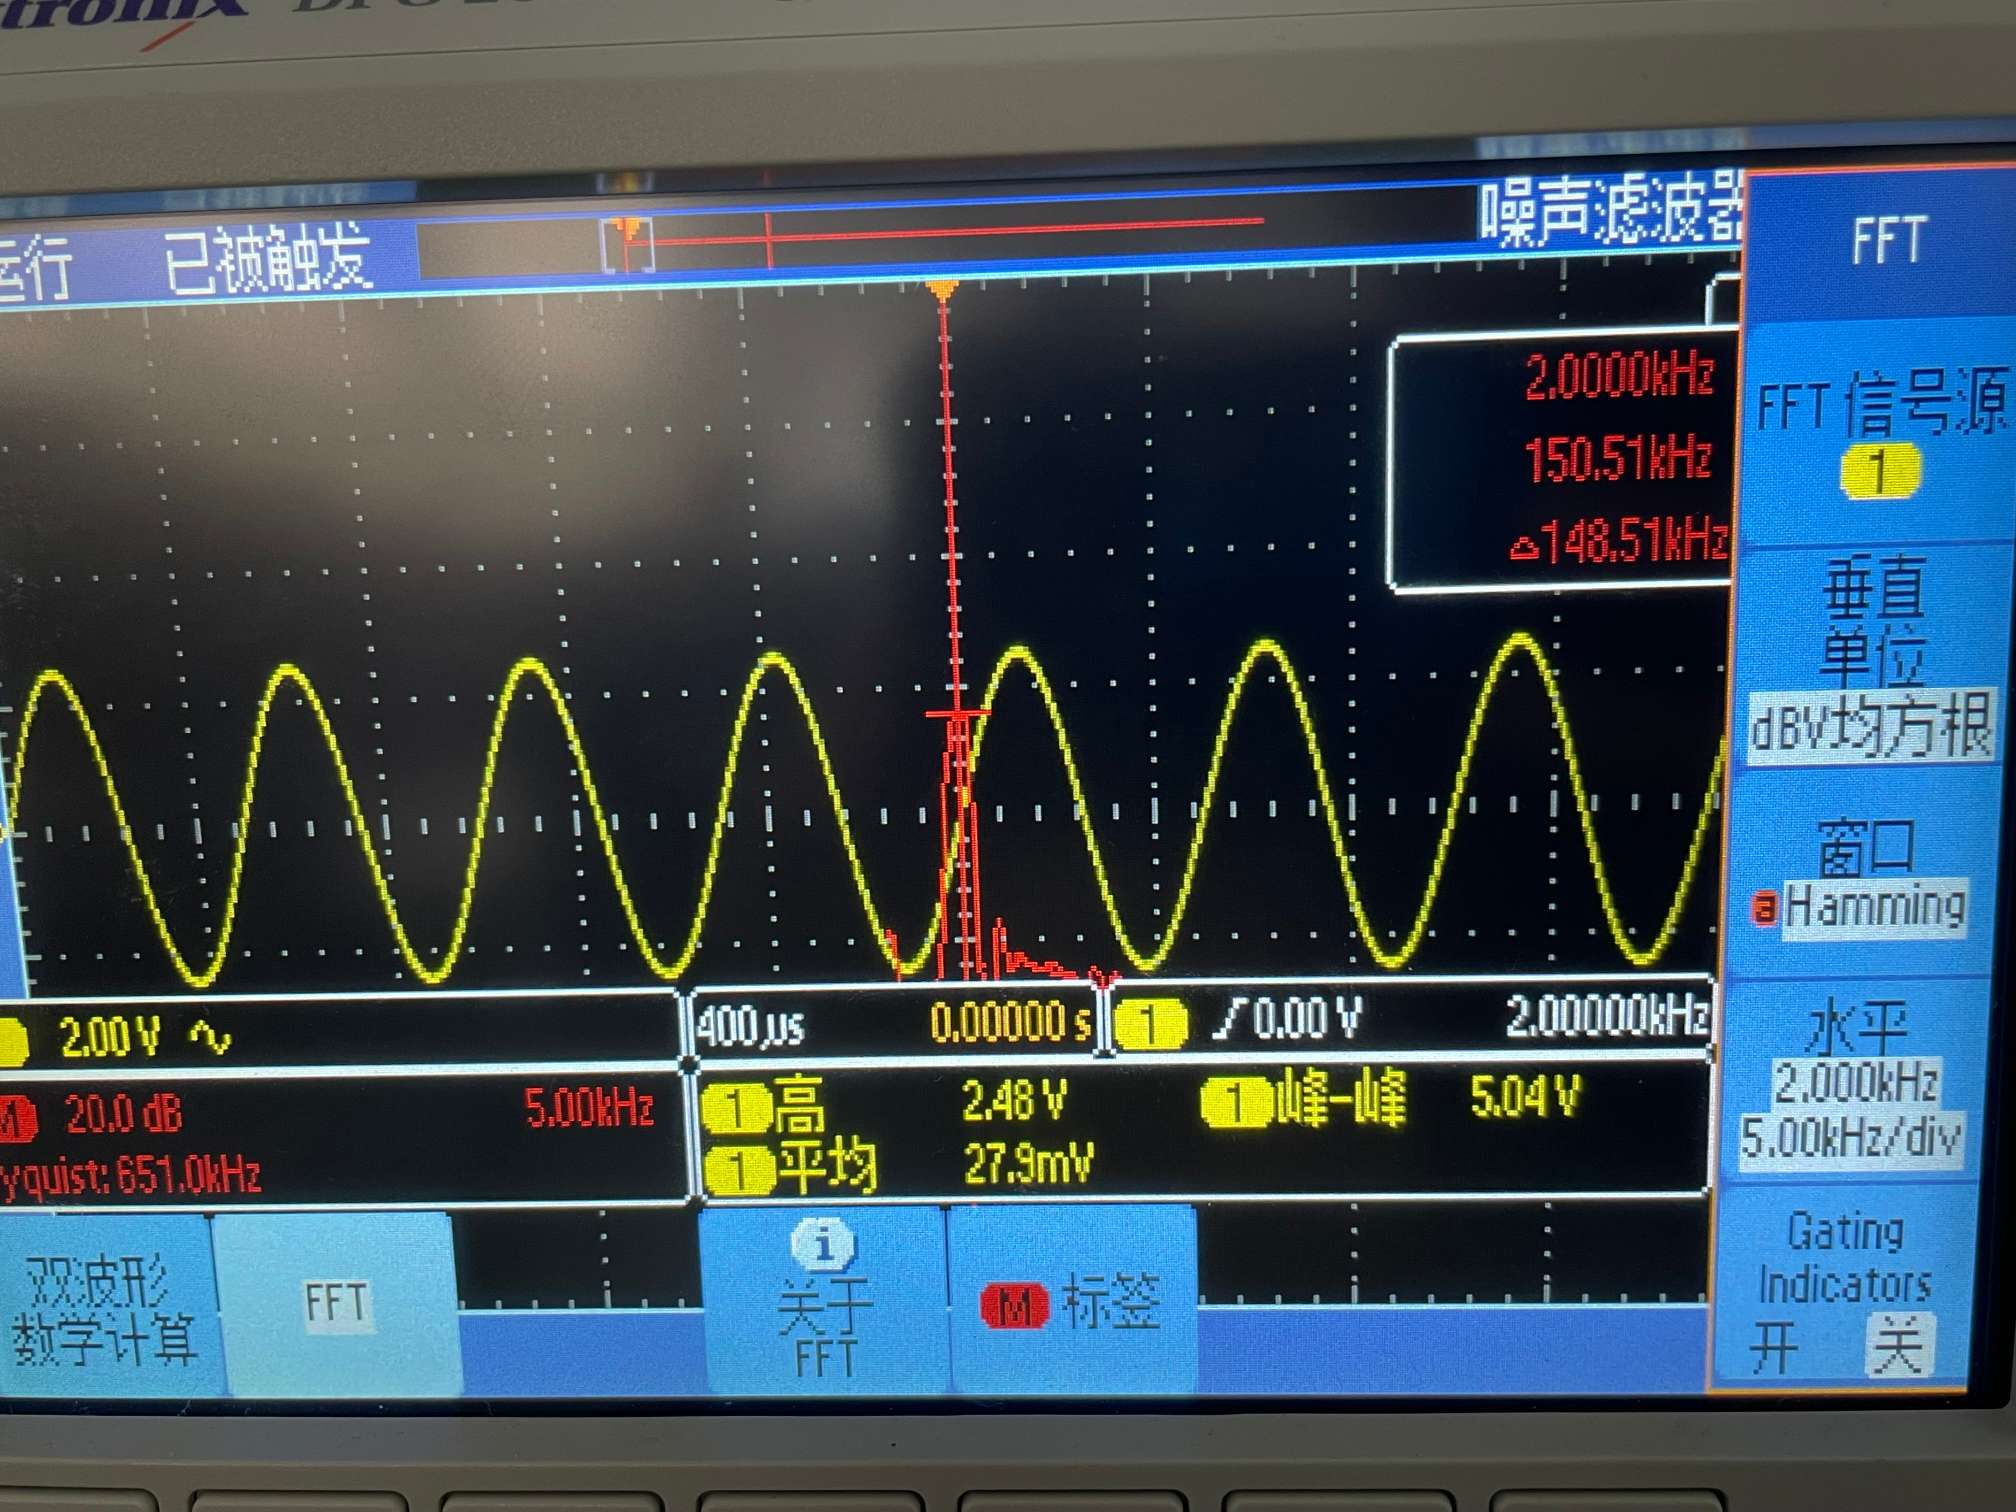
\includegraphics[width=0.3\textwidth]{hamming_sine_osc_2.jpg}
    }
     \hspace{0.005\linewidth}
      \subfigure[subfigure 1-2][汉宁窗频谱测量]{
        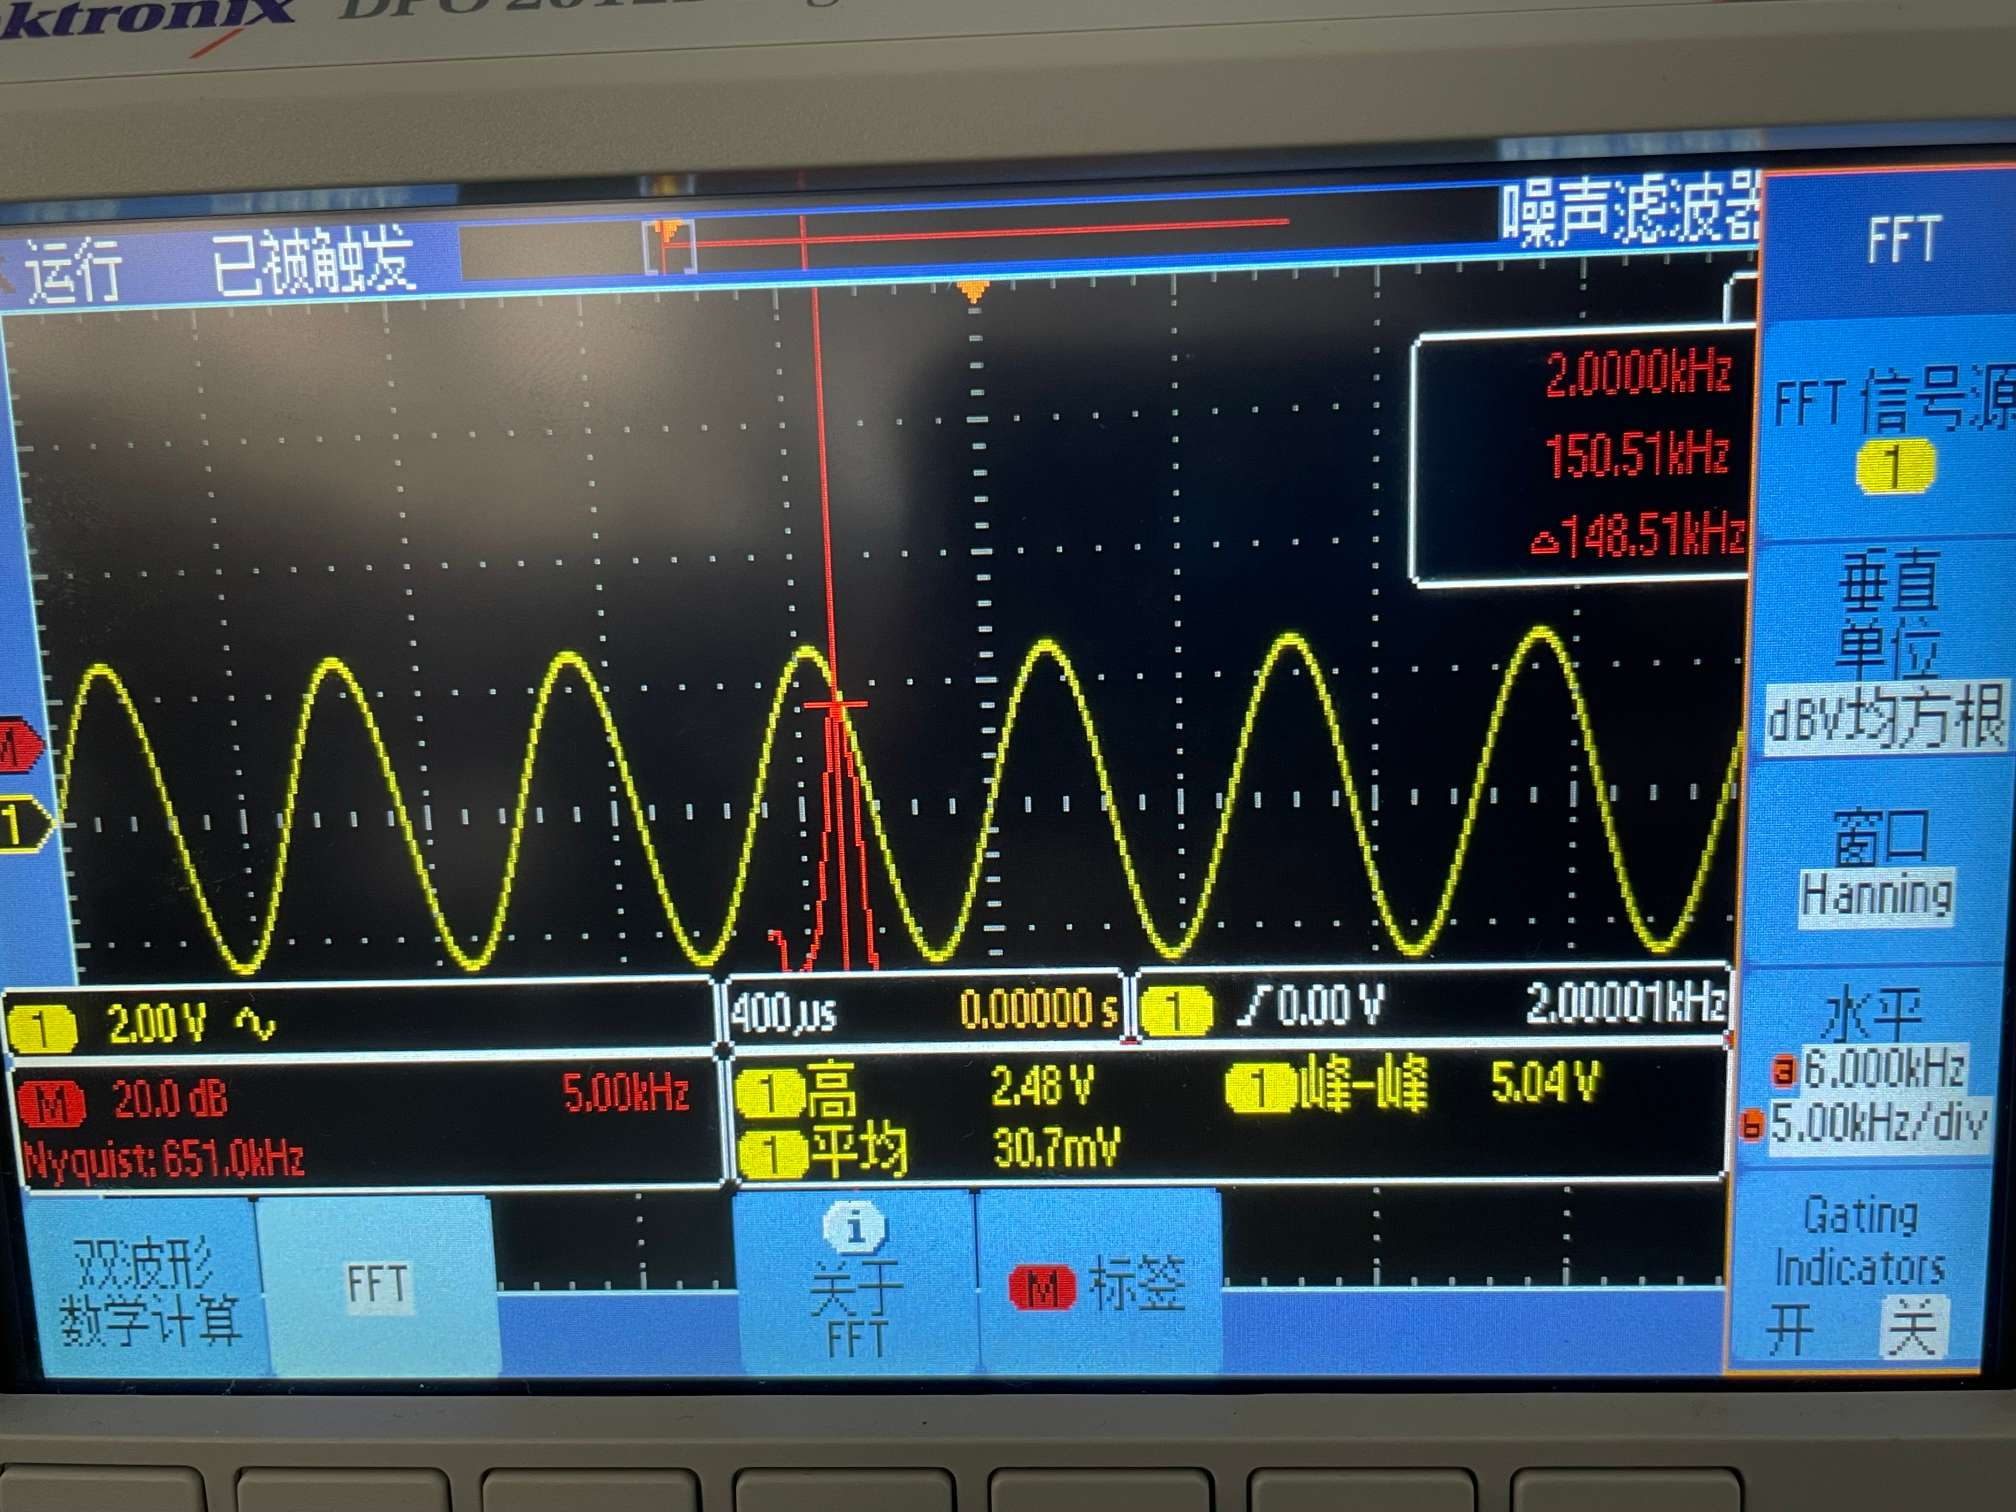
\includegraphics[width=0.3\textwidth]{hanning_sine_osc_2.jpg}
    }
         \hspace{0.005\linewidth}
      \subfigure[subfigure 1-3][矩形窗频谱]{
        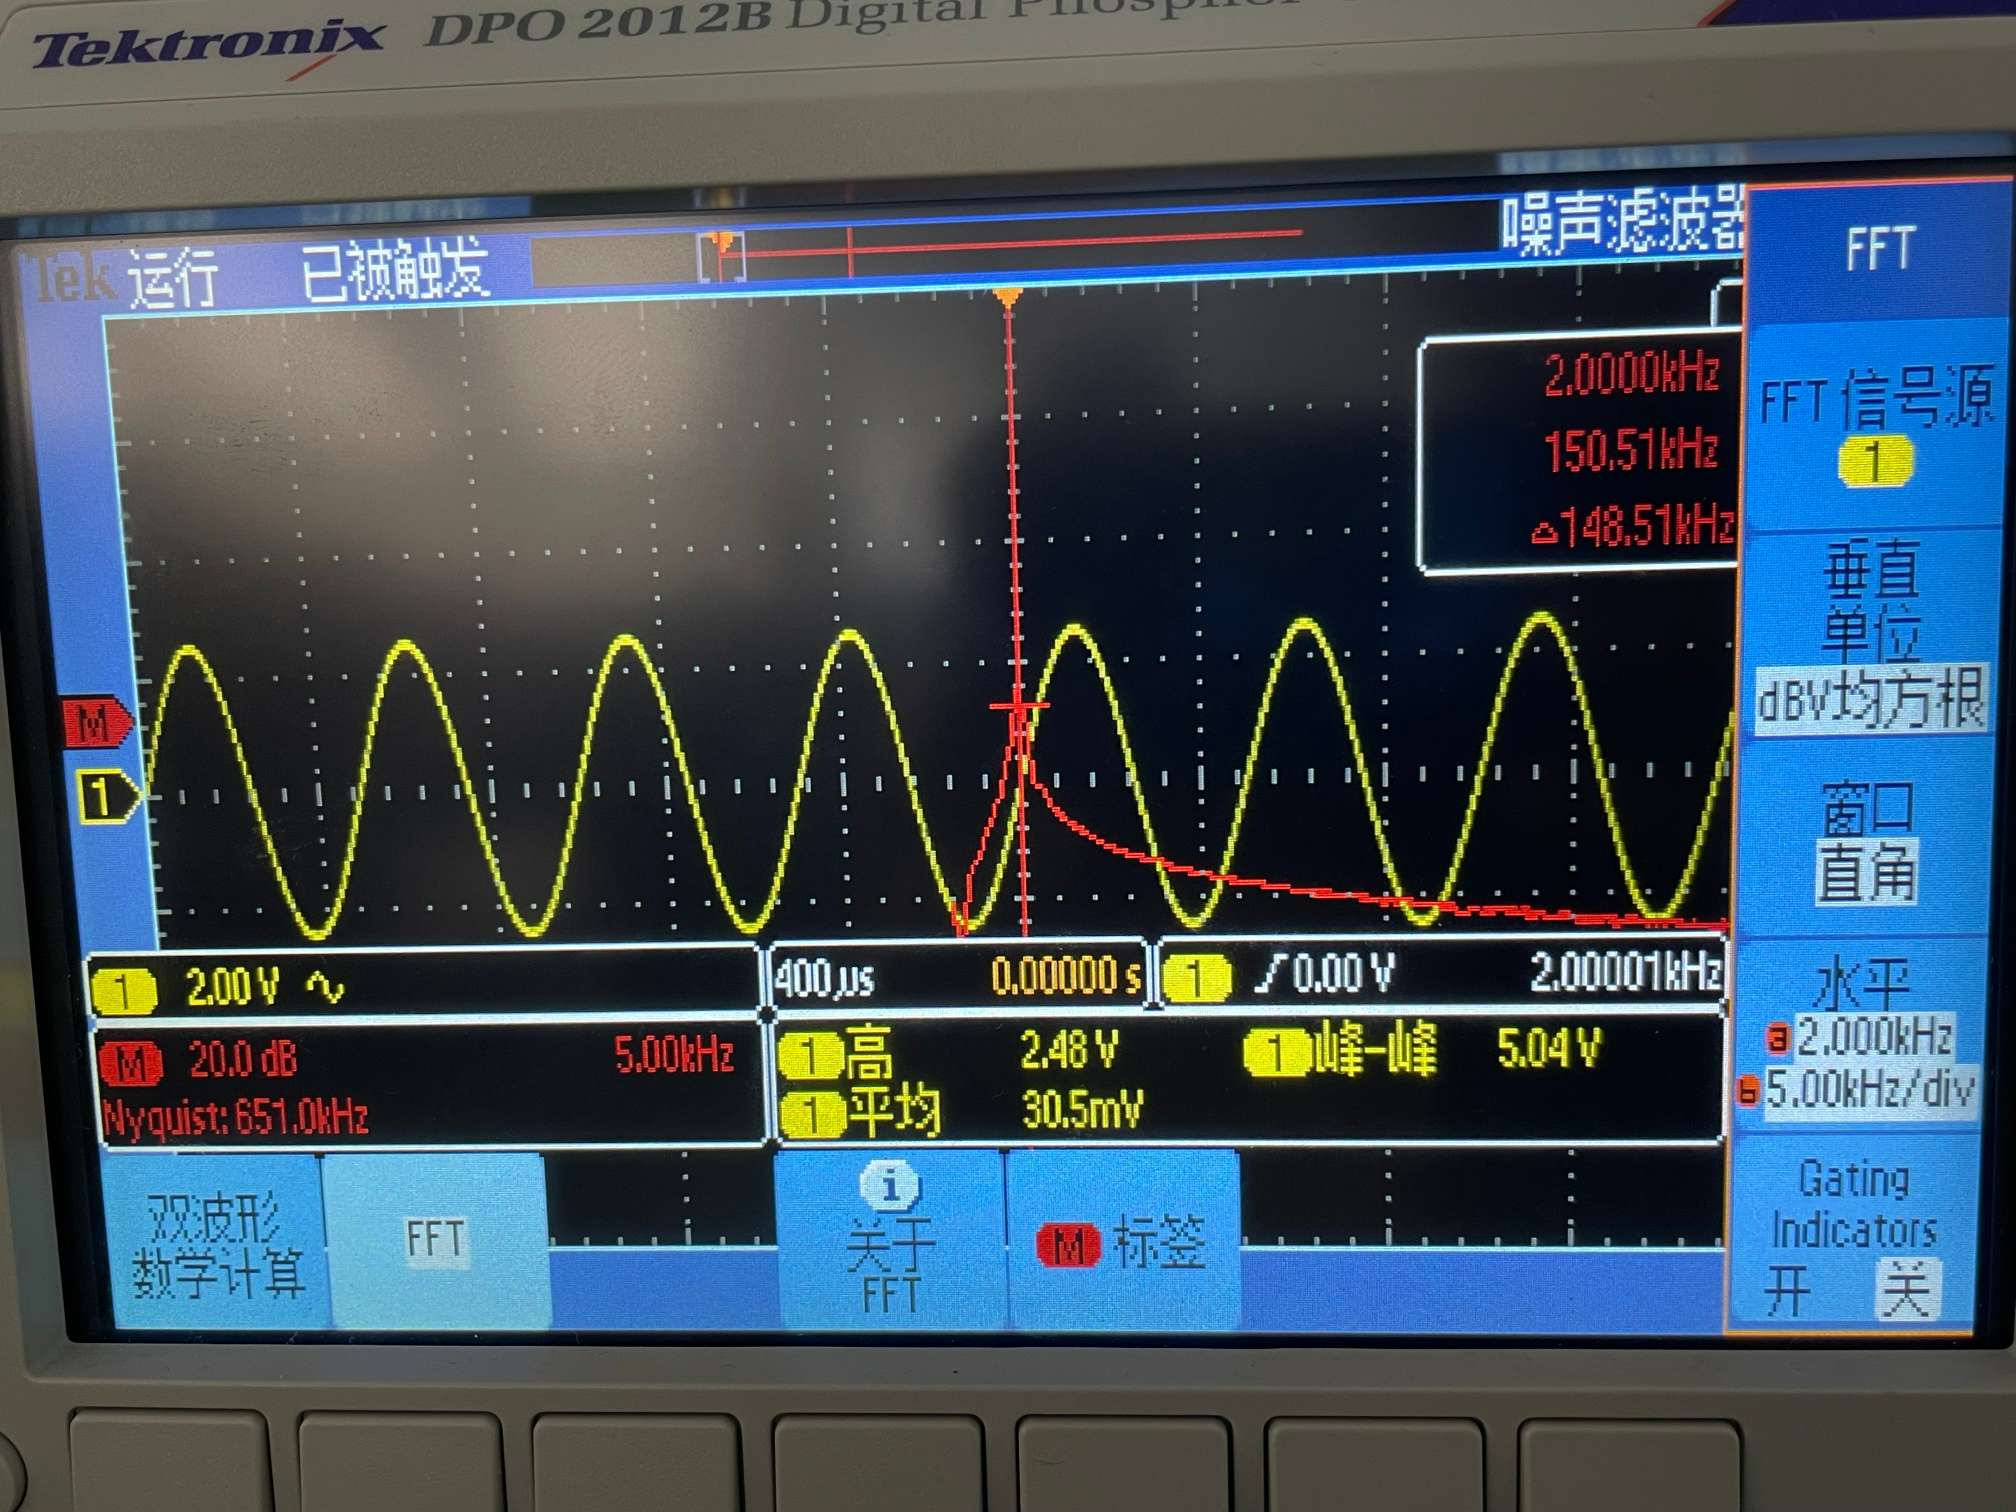
\includegraphics[width=0.3\textwidth]{rect_sine_osc_2.jpg}
    }
    \caption{示波器测量正弦单音信号时频域波形}
  \label{示波器1a(2)}
\end{figure}

\subsubsection{示波器测量单音正弦信号结果分析}
如图\ref{示波器1a}所示,三种窗函数下的FFT频谱在2kHz频点上均存在尖峰,但三种窗函数存在不同程度的频谱能量泄露。观察图\ref{示波器1a}(c),矩形窗的衰减最弱\footnote{矩形窗可看作理想低通滤波器,对经FFT处理信号的不连续点不产生衰减。},频谱幅度分辨率很低,高频部分幅值较大,这是由于矩形窗的旁瓣较高,并且有负旁瓣,导致变换过程中引入了高频干扰和较大的频谱泄漏。但经矩形窗变换的正弦信号具有较尖的峰值,这是由于在三种窗中,矩形窗有较窄的主瓣宽度,使单音信号的频率读取更为容易。

汉明窗及汉宁窗都为升余弦窗,相比矩形窗,两者的第一旁瓣衰减高,因此频谱集中程度高,在示波器频谱上体现为2kHz峰值明显,两侧的频谱幅值迅速衰减。两者的区别在于,汉明窗的第一旁瓣衰减(-42dB)快于汉宁窗,而第二、第三等旁瓣衰减速度慢于汉宁窗,因此示波器中观察到相对汉宁窗,汉明窗对应的FFT频谱在高频部分也存在较小的峰。

因此,矩形窗具有更高的频率分辨力。但频谱泄漏严重;汉宁窗在高频干扰与漏能的消除上上最优的;汉明窗的主瓣衰减较快,选出了被测信号的频域峰值,在频谱泄漏的消除上略弱于汉宁窗。



\subsubsection{M2K测量单音正弦信号}


\textbf{实验要求b}:用M2K产生一个 2KHz 的正弦波,并用M2K中的
示波器和频谱仪观测信号,重复a)中的实验项目。

\textbf{实验过程}:将排针插入ADALM2000杜邦线孔内做成探头。其中,1-端接地,1+端接W1,接入计算机设备后,运行SCOPY。在SCOPY界面,点击Signal Generator,将波的类型设置为Sine,频率设为2kHz。点击运行按钮。

点击Spectrum Analyzer,设置显示中心频率为5kHz,频谱跨度10kHz。依次选择汉明窗、汉宁窗、矩形窗后,点击运行按钮,观察到频谱如下:
\begin{figure}[H]
    \centering
    
    \subfigure[subfigure 1-1][汉明窗频谱测量]{
        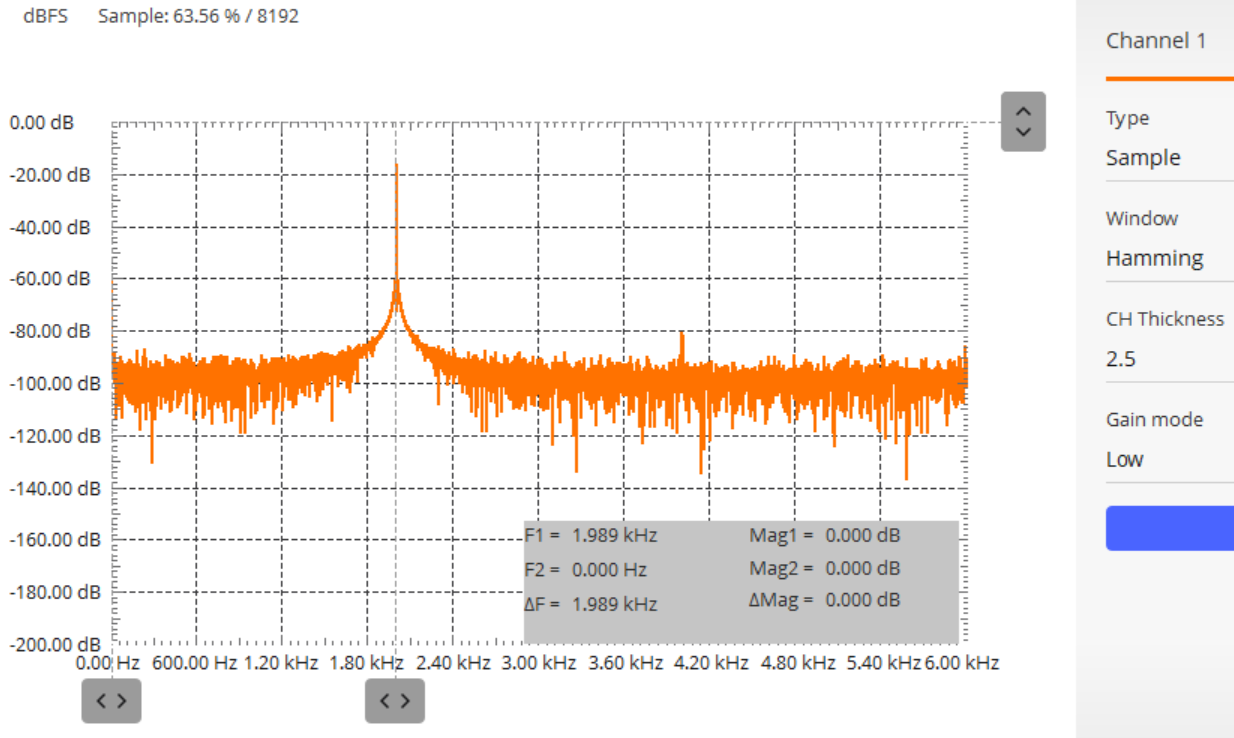
\includegraphics[width=0.3\textwidth]{scopy_sine_hamming.png}
    }
     \hspace{0.005\linewidth}
      \subfigure[subfigure 1-2][汉宁窗频谱测量]{
        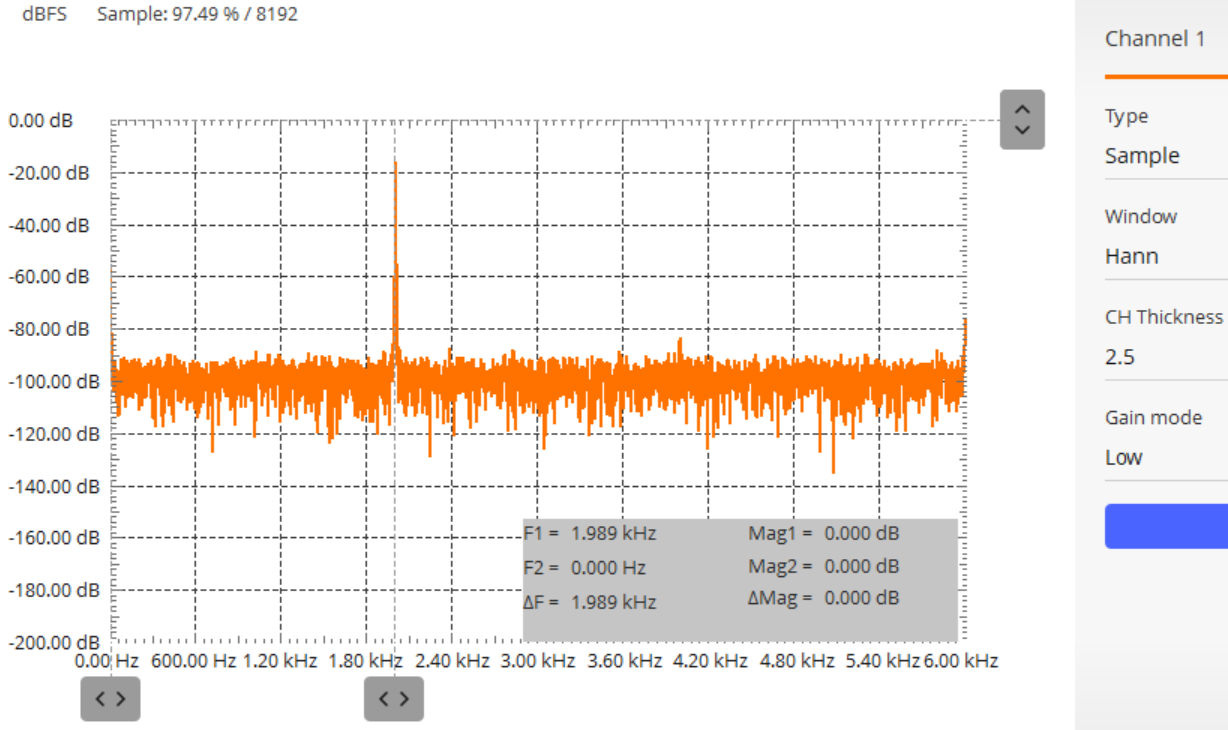
\includegraphics[width=0.3\textwidth]{scopy_sine_hann.png}
    }
         \hspace{0.005\linewidth}
      \subfigure[subfigure 1-3][矩形窗频谱]{
        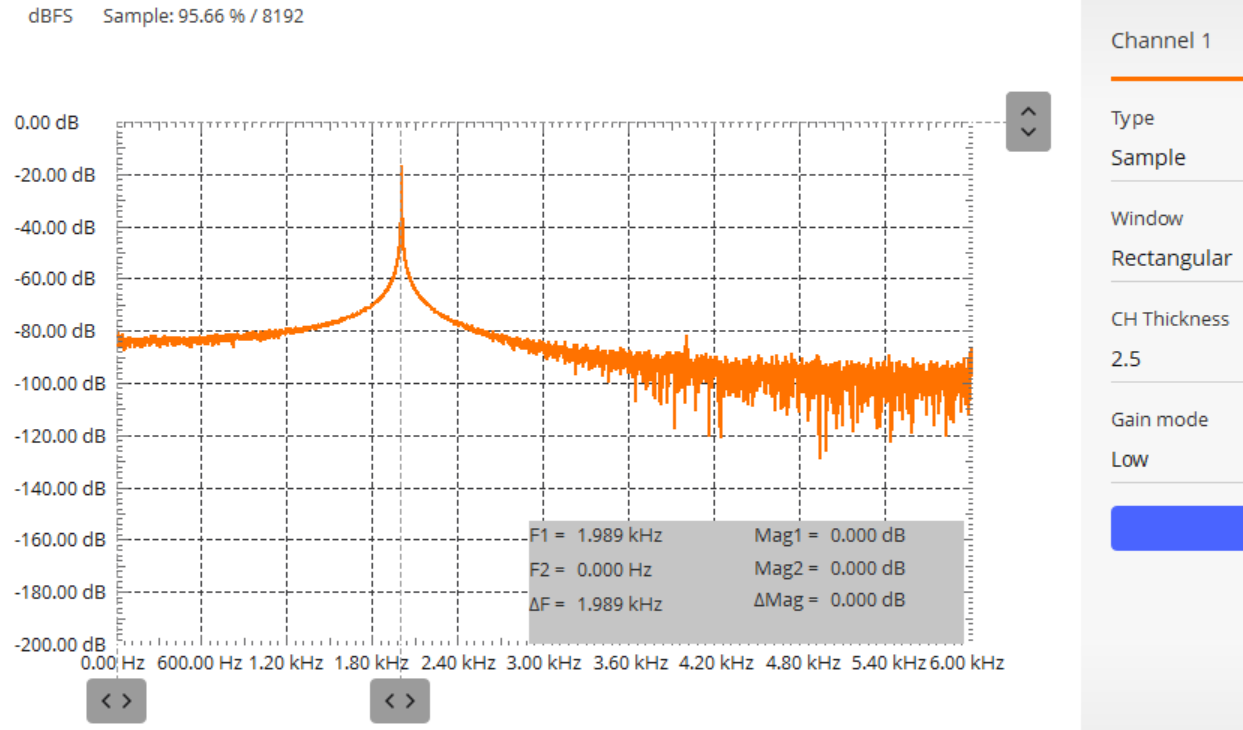
\includegraphics[width=0.3\textwidth]{scopy_sine_rect.png}
    }
    \caption{Scopy测量正弦单音信号频域波形}
  \label{Scopy_sine}
\end{figure}

如图\ref{Scopy_sine}所示,在三个子图中,均能看到2kHz频点上有明显的峰,矩形窗的幅度分辨率相对最弱。汉宁窗的频谱泄漏程度最小,除2kHz外的频点幅值迅速下降。汉明窗的衰减程度也较高,但不及汉宁窗明显。


\subsubsection{MATLAB编程实现单音正弦信号幅度谱}

\textbf{实验要求c}:利用 MATLAB 产生2KHz 的正弦波,用不同
宽度的窗函数进行截断,通过编程绘制出其幅度谱,
并说明其与宽度变化的关系,并说明与a),b)中的
差别及其原因。

\textbf{实验过程}:编写程序,根据表\ref{window}构造三种窗函数,傅里叶变换部分采用向量乘积法,核心代码如下\footnote{为精简起见,将绘图部分代码省略,下同。}:
\begin{lstlisting}
        clear;clc;
        f = 2000;
        t1 = 0; t2 = 0.0025; %t1不变,t2选择0.0025,0.025及0.25以测试不同窗长对频谱的影响
        f1 = 0; f2 = 3000; df = 1;
        T = t2 - t1; dt = T / 10000; %dt:时间精度
        t = t1:dt:t2;
        x = sin(2 * pi * f * t);
        N = T / dt; %N:采样点数
        hn = hanning(N + 1); hm = hamming(N + 1); w = boxcar(N + 1); %三种窗函数,hn:汉宁窗;hm:汉明窗;w:矩形窗
        F1 = [];F2 = [];F3 = []; %频域函数
    
        count = 0;
        for k = f1:df:f2 %向量法写傅里叶变换
            t_1 = exp(-1j * 2 * pi * k * t);
            count = count + 1;
            F1(count) = abs(T / N * t_1 * (x' .* hm));
            F2(count) = abs(T / N * t_1 * (x' .* hn));
            F3(count) = abs(T / N * t_1 * (x' .* w));
        end
\end{lstlisting}

MATLAB实验结果如下所示:
\begin{figure}[H]
    \centering
    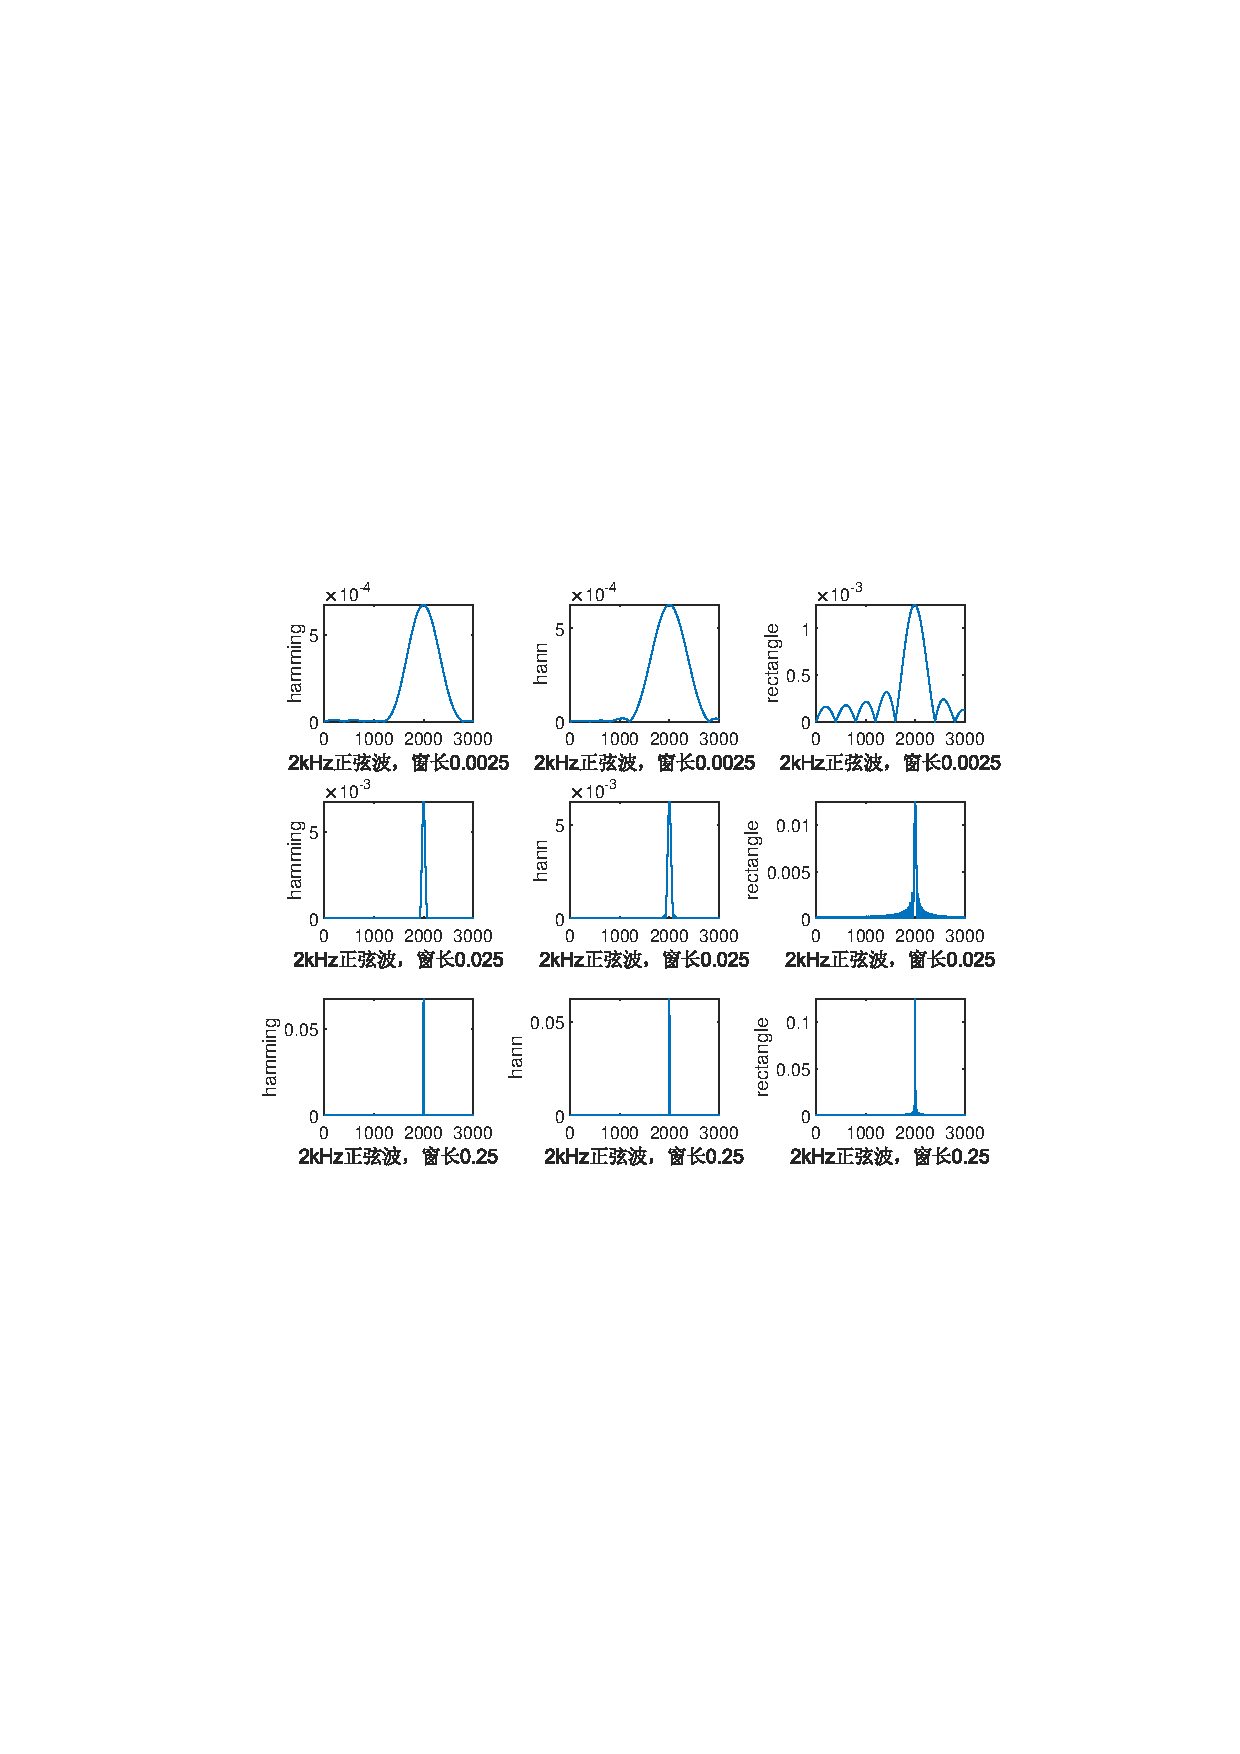
\includegraphics[scale=1]{matlab_sine.pdf}
    \caption{MATLAB加窗绘制单音正弦信号(2kHz)频谱}
    \label{MATLAB_sin}
\end{figure}

\subsubsection{窗函数宽度与单音正弦信号幅度谱的关系}
如图\ref{MATLAB_sin},纵向对比同种窗函数下幅度谱的变化,但窗函数从0.0025增至0.025,再增至0.25,幅度谱宽度逐渐减小,并逐渐接近单音信号的冲激函数形式$\delta(f-2000)$。即窗函数加宽,中心频率以外的频率分量衰减更快,频谱的泄露程度减小。

以矩形窗$\omega(t)$为例,假定矩形窗的窗长为$T$,输入任意信号x(t),截断信号为$x_{T}(t)$,则
\begin{center}
{\setlength\abovedisplayskip{-0.3cm}
    \begin{equation}
        \begin{aligned}
        \omega(t)=&\mathrm{rect}\frac{t}{T}\\
        x_{T}(t)=&x(t)\cdot \omega(t)\\
        \Rightarrow X_{T}(\omega)=&\frac{1}{2\pi}X(\omega)*W(\omega)\\
        =& \frac{1}{2\pi}X(\omega)* T\mathrm{Sa}(\frac{T\omega}{2})\\
        \end{aligned}
    \end{equation}
    }
    \label{omega}
\end{center}
由于此处$x(t)$频谱为冲激函数,从而$X_{T}(\omega)$频谱仍保留$\mathrm{Sa}()$函数性质。对主瓣零点$\pi$,对应角频率$\omega_{0}=\frac{2\pi}{T}$。由此可知,窗函数宽度$T$增加,零点减小,衰减加快。

同时,窗函数宽度增加,2kHz频点幅度谱的幅值升高,对应能量更集中。

\subsubsection{MATLAB仿真与示波器、Scopy测量正弦波的对比分析}
\begin{itemize}
    \item 产生信号的差异:MATLAB仿真在取样点数足够多、窗函数足够宽的情况下,幅度谱近似为单一频点的冲激函数,而示波器和M2K产生信号在非频点处有大量毛刺,其原因在于:MATLAB仿真忽略了现实环境因素,例如仪器底噪和白噪声;而示波器和M2K均是物理信号源输入,含有仪器底噪和环境白噪声,噪声使得波形显示出现大量毛刺。
    \item 频点的差异:示波器与M2K均出现了50Hz的频谱,这是受到50Hz市电干扰产生,因此使用该电源的设备均会带有这个频率的分量;而MATLAB为软件仿真结果,不存在50Hz干扰。
    \item 频率分辨率的差异:采用示波器观察信号时,频率分辨率需手动调节,且初始测量时频率分辨率较低,这由时基宽度决定,一般地,示波器分辨率带宽 = 1 / (时基长度$\times$水平格子数);而用M2K自动测量时,初始频率分辨率较高,无需后期调节,如图\ref{Scopy_sine}所示,可观察到2kHz频点处信号能量集中;用MATLAB仿真时,频谱宽度则主要依靠调节窗长改变。
    \item 幅度的差异:窗长固定时,采用不同窗函数,MATLAB仿真对应的幅度谱幅值发生改变;而示波器、M2K测量得到的幅度谱幅值不变。这是由于MATLAB仿真采用的是傅里叶变换,其运算结果的幅值受窗函数类型的影响;而示波器、M2K采用FFT变换,幅值不受窗函数类型影响。
\end{itemize}














\subsection{实验二:2kHz方波}
\subsubsection{示波器测量方波信号}
\textbf{实验要求a}:用波形发生器产生一个2kHz的周期方波,用示波器观察其时域波形并记录;用FFT功能观察频谱并记录;采用几种窗函数形式记录频谱,并分析其变化原因。

\textbf{实验过程}:将信号发生器设为2kHz,峰峰值为5V的方波信号,待示波器波形稳定后,旋转示波器水平旋钮,使屏幕上显示尽可能多的方波周期。按下Math模式,按下FFT功能,按下水平按键,并将精度调至2.50kHz/div。当时域周期数逐渐增多时,观察到谱线峰值逐渐明显,且非峰值区域变宽,幅值减小。此时按下Menu off,并利用光标法测得其相邻峰值频点间隔约4.0kHz。

实验结果测量如下:
\begin{figure}[H]
    \centering
    
    \subfigure[subfigure 1-1][矩形窗频谱测量]{
        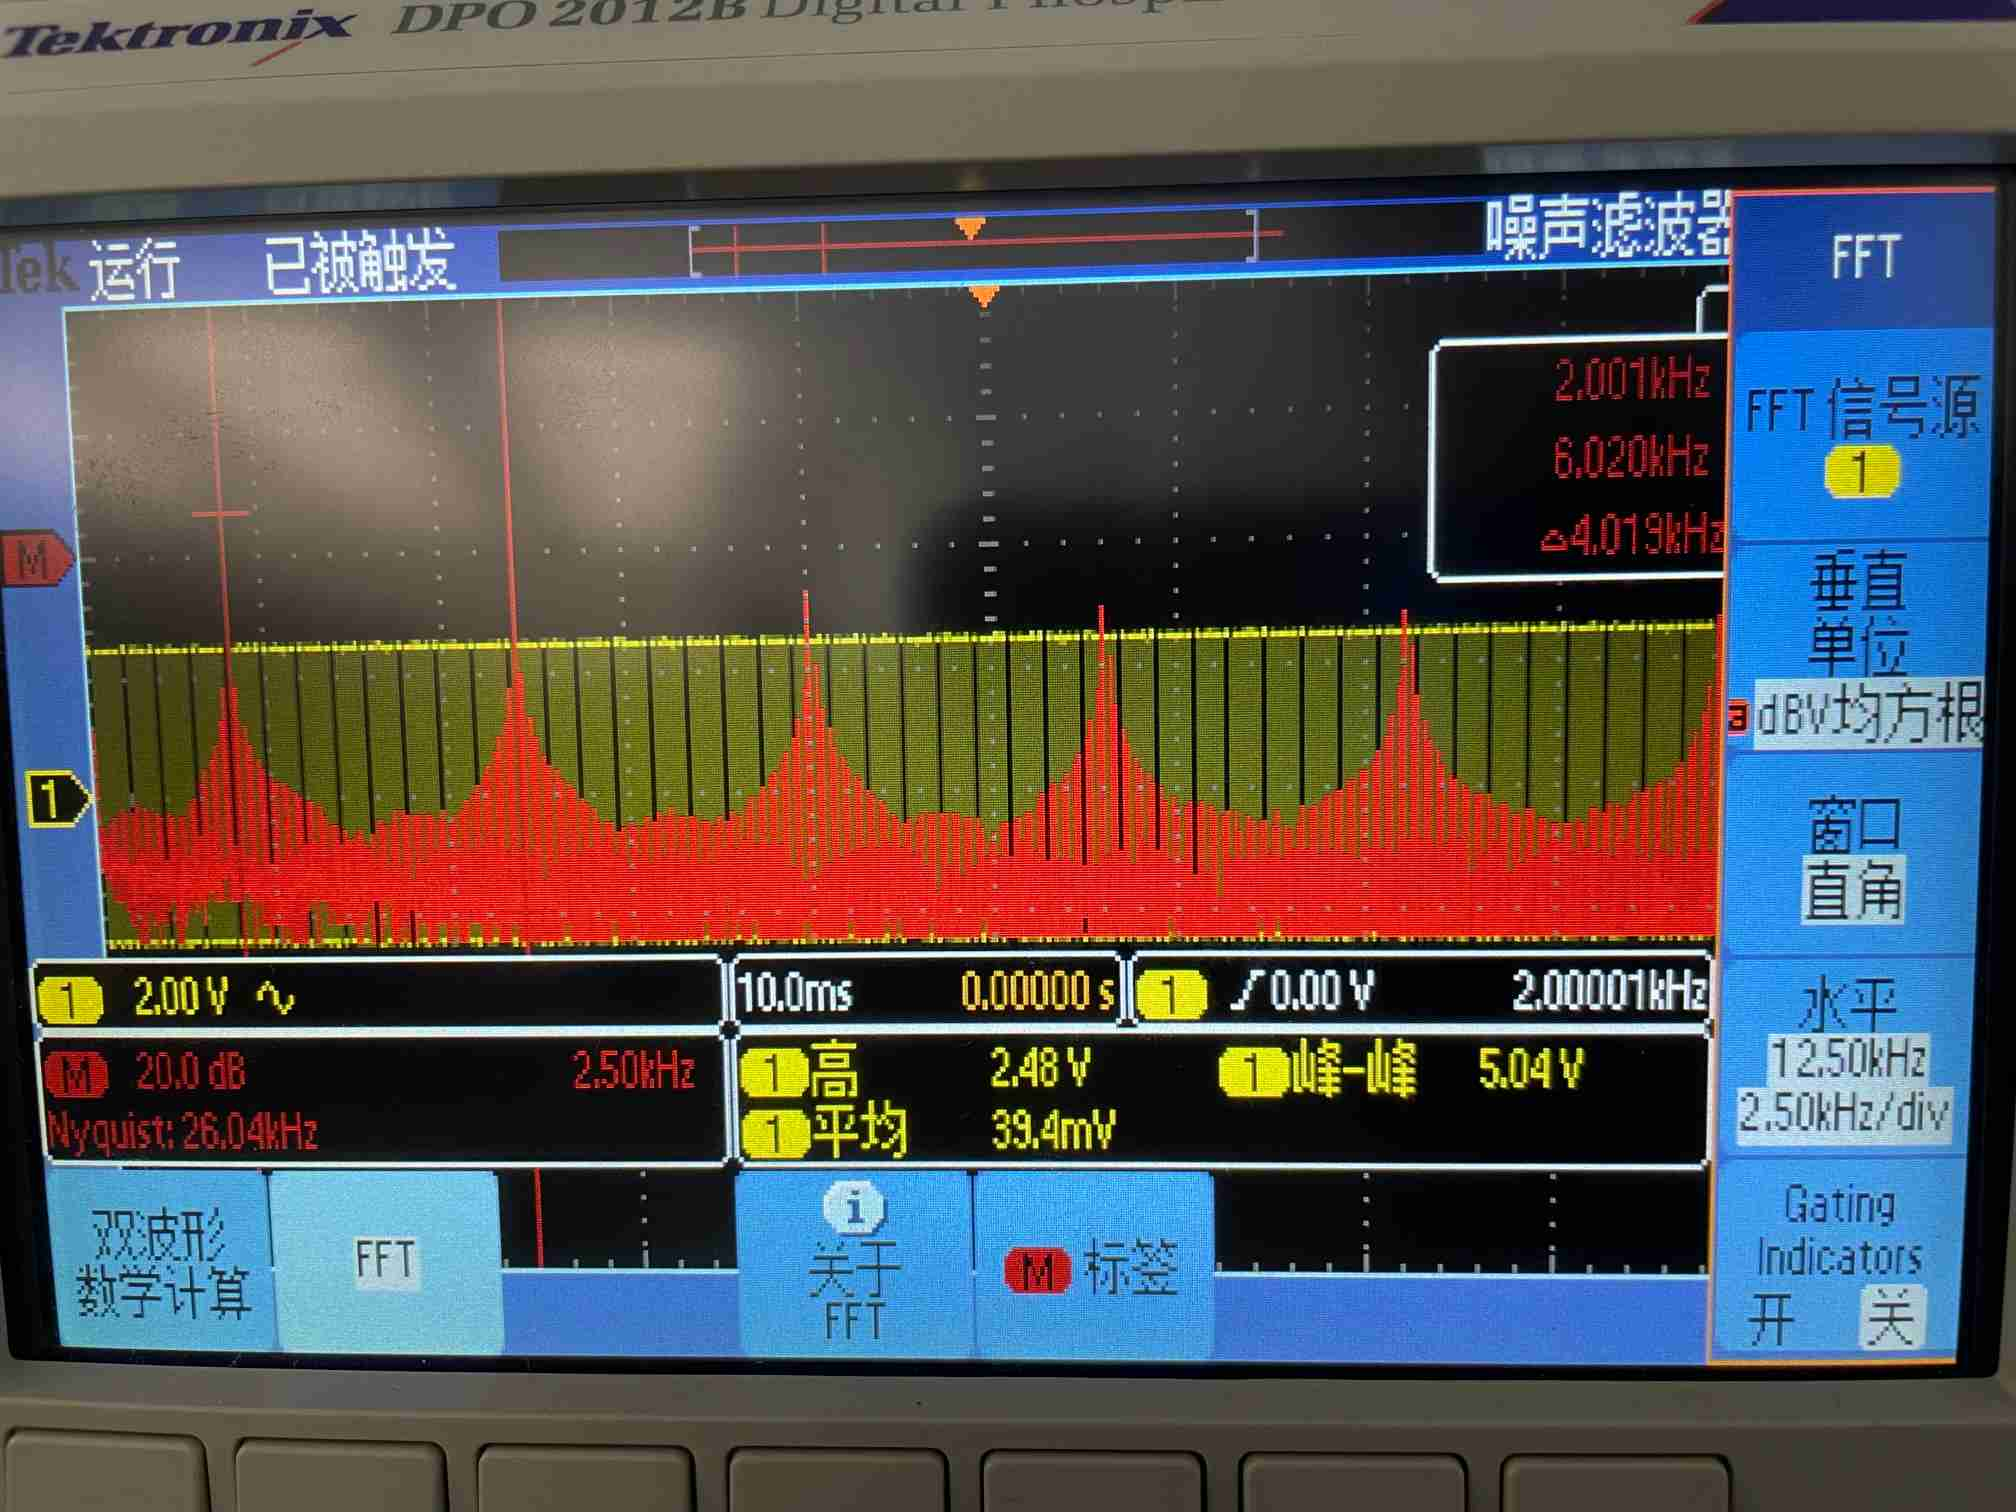
\includegraphics[width=0.3\textwidth]{rect_squ_osc.jpg}
    }
     \hspace{0.005\linewidth}
      \subfigure[subfigure 1-2][Blackman-Harris窗频谱测量]{
        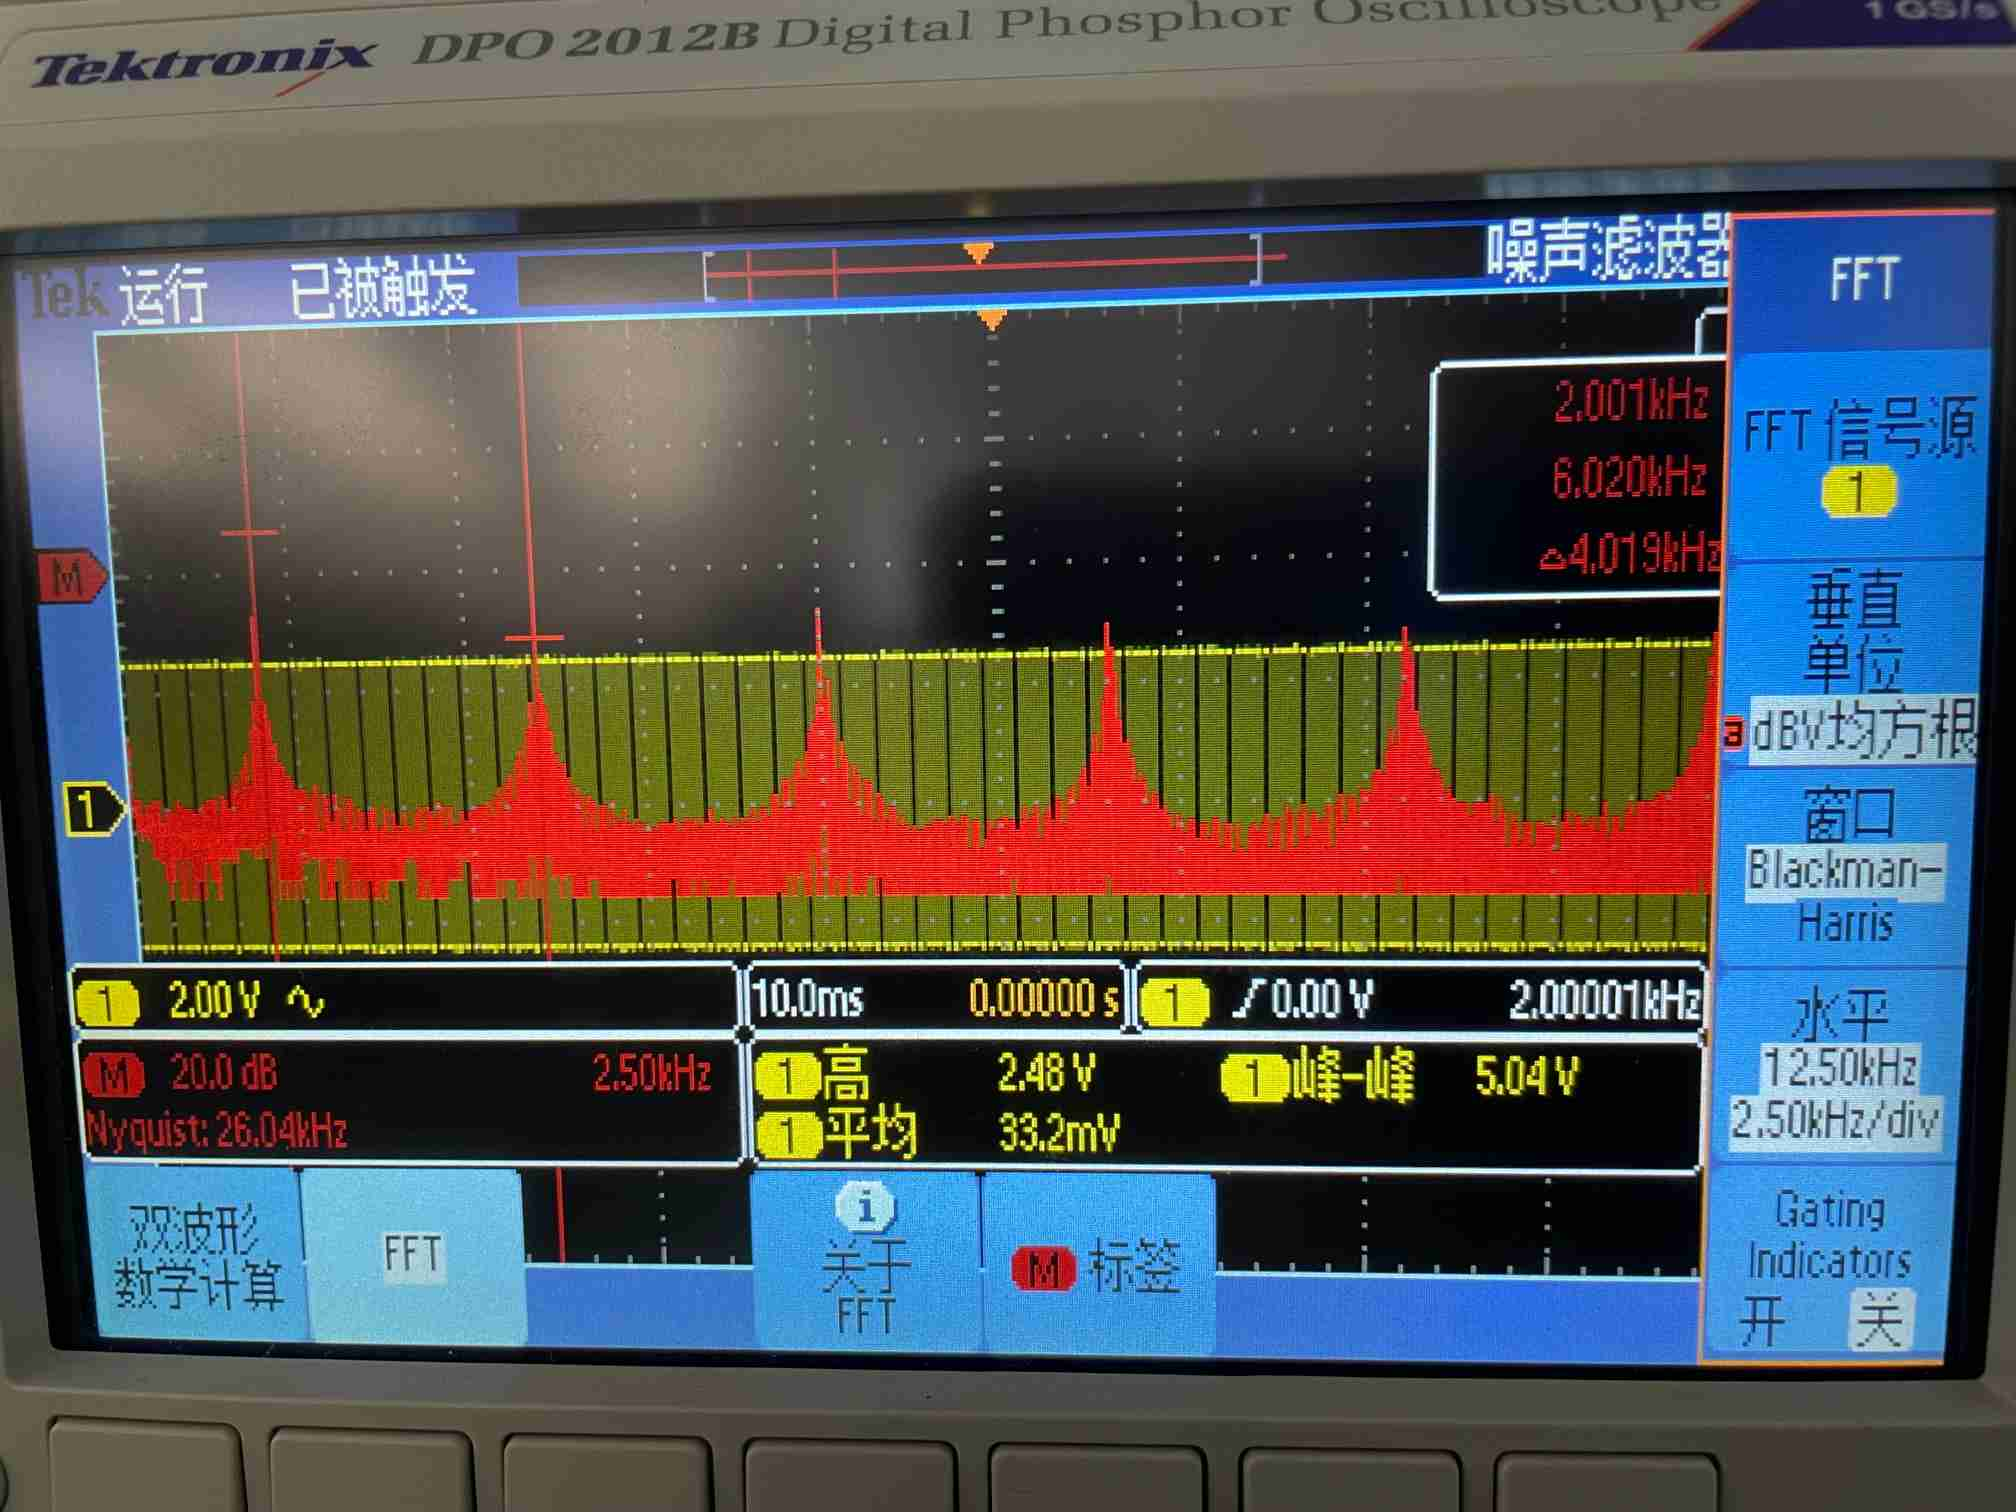
\includegraphics[width=0.3\textwidth]{black_squ_osc.jpg}
    }
       
      \subfigure[subfigure 2-1][汉明窗频谱测量]{
        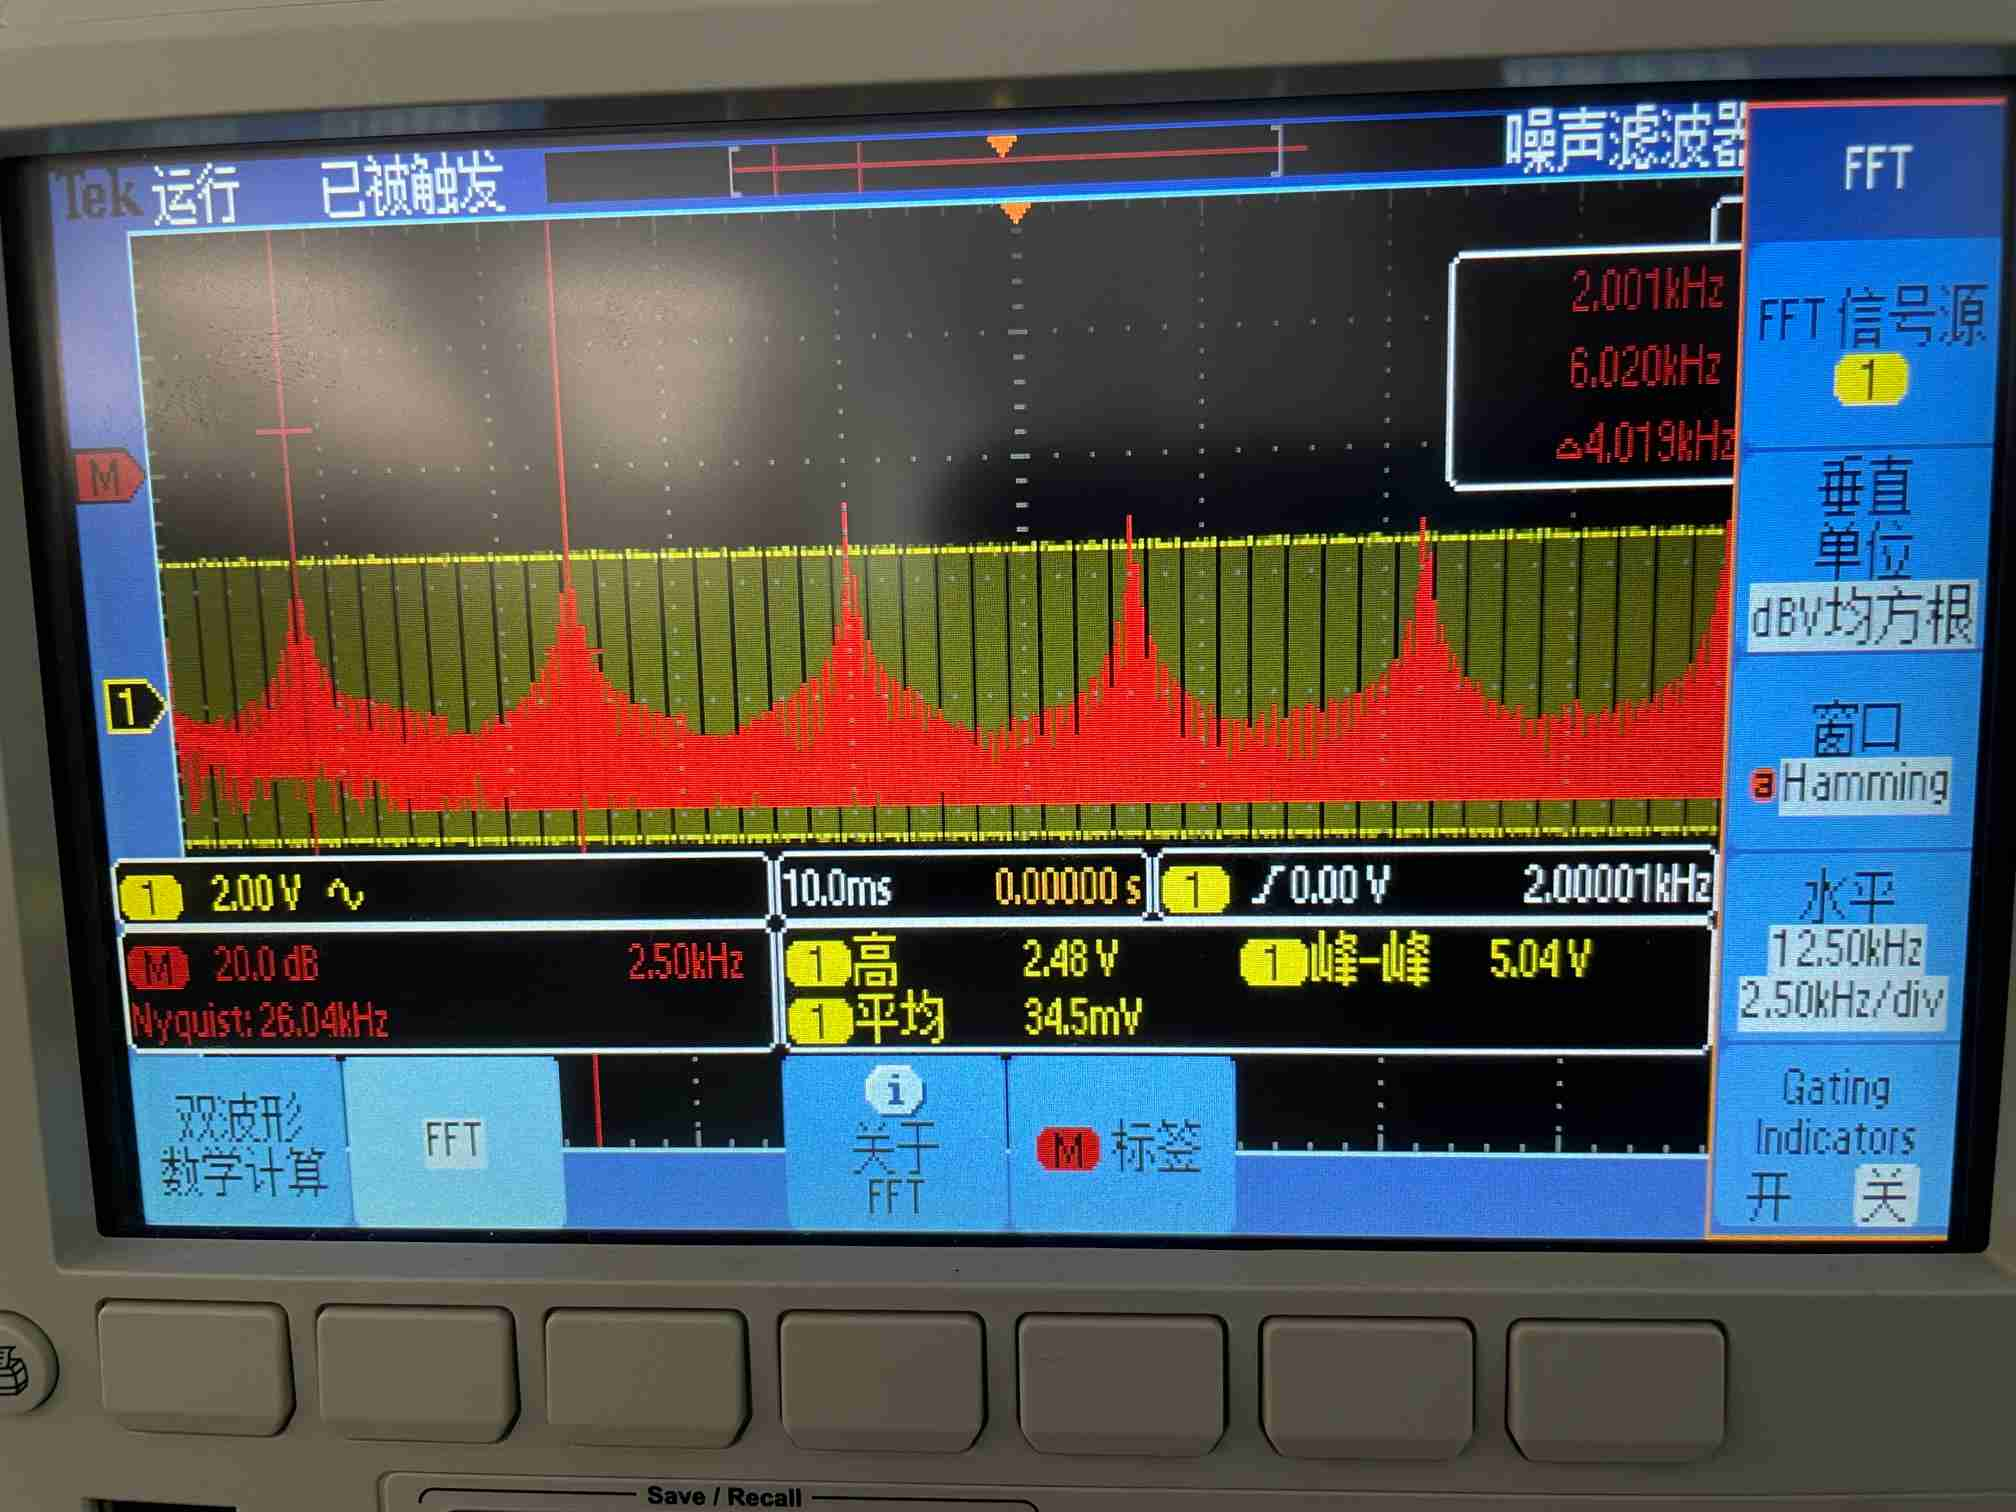
\includegraphics[width=0.3\textwidth]{hamming_squ_osc.jpg}
    }
    \hspace{0.005\linewidth}
          \subfigure[subfigure 2-1][汉宁窗频谱测量]{
        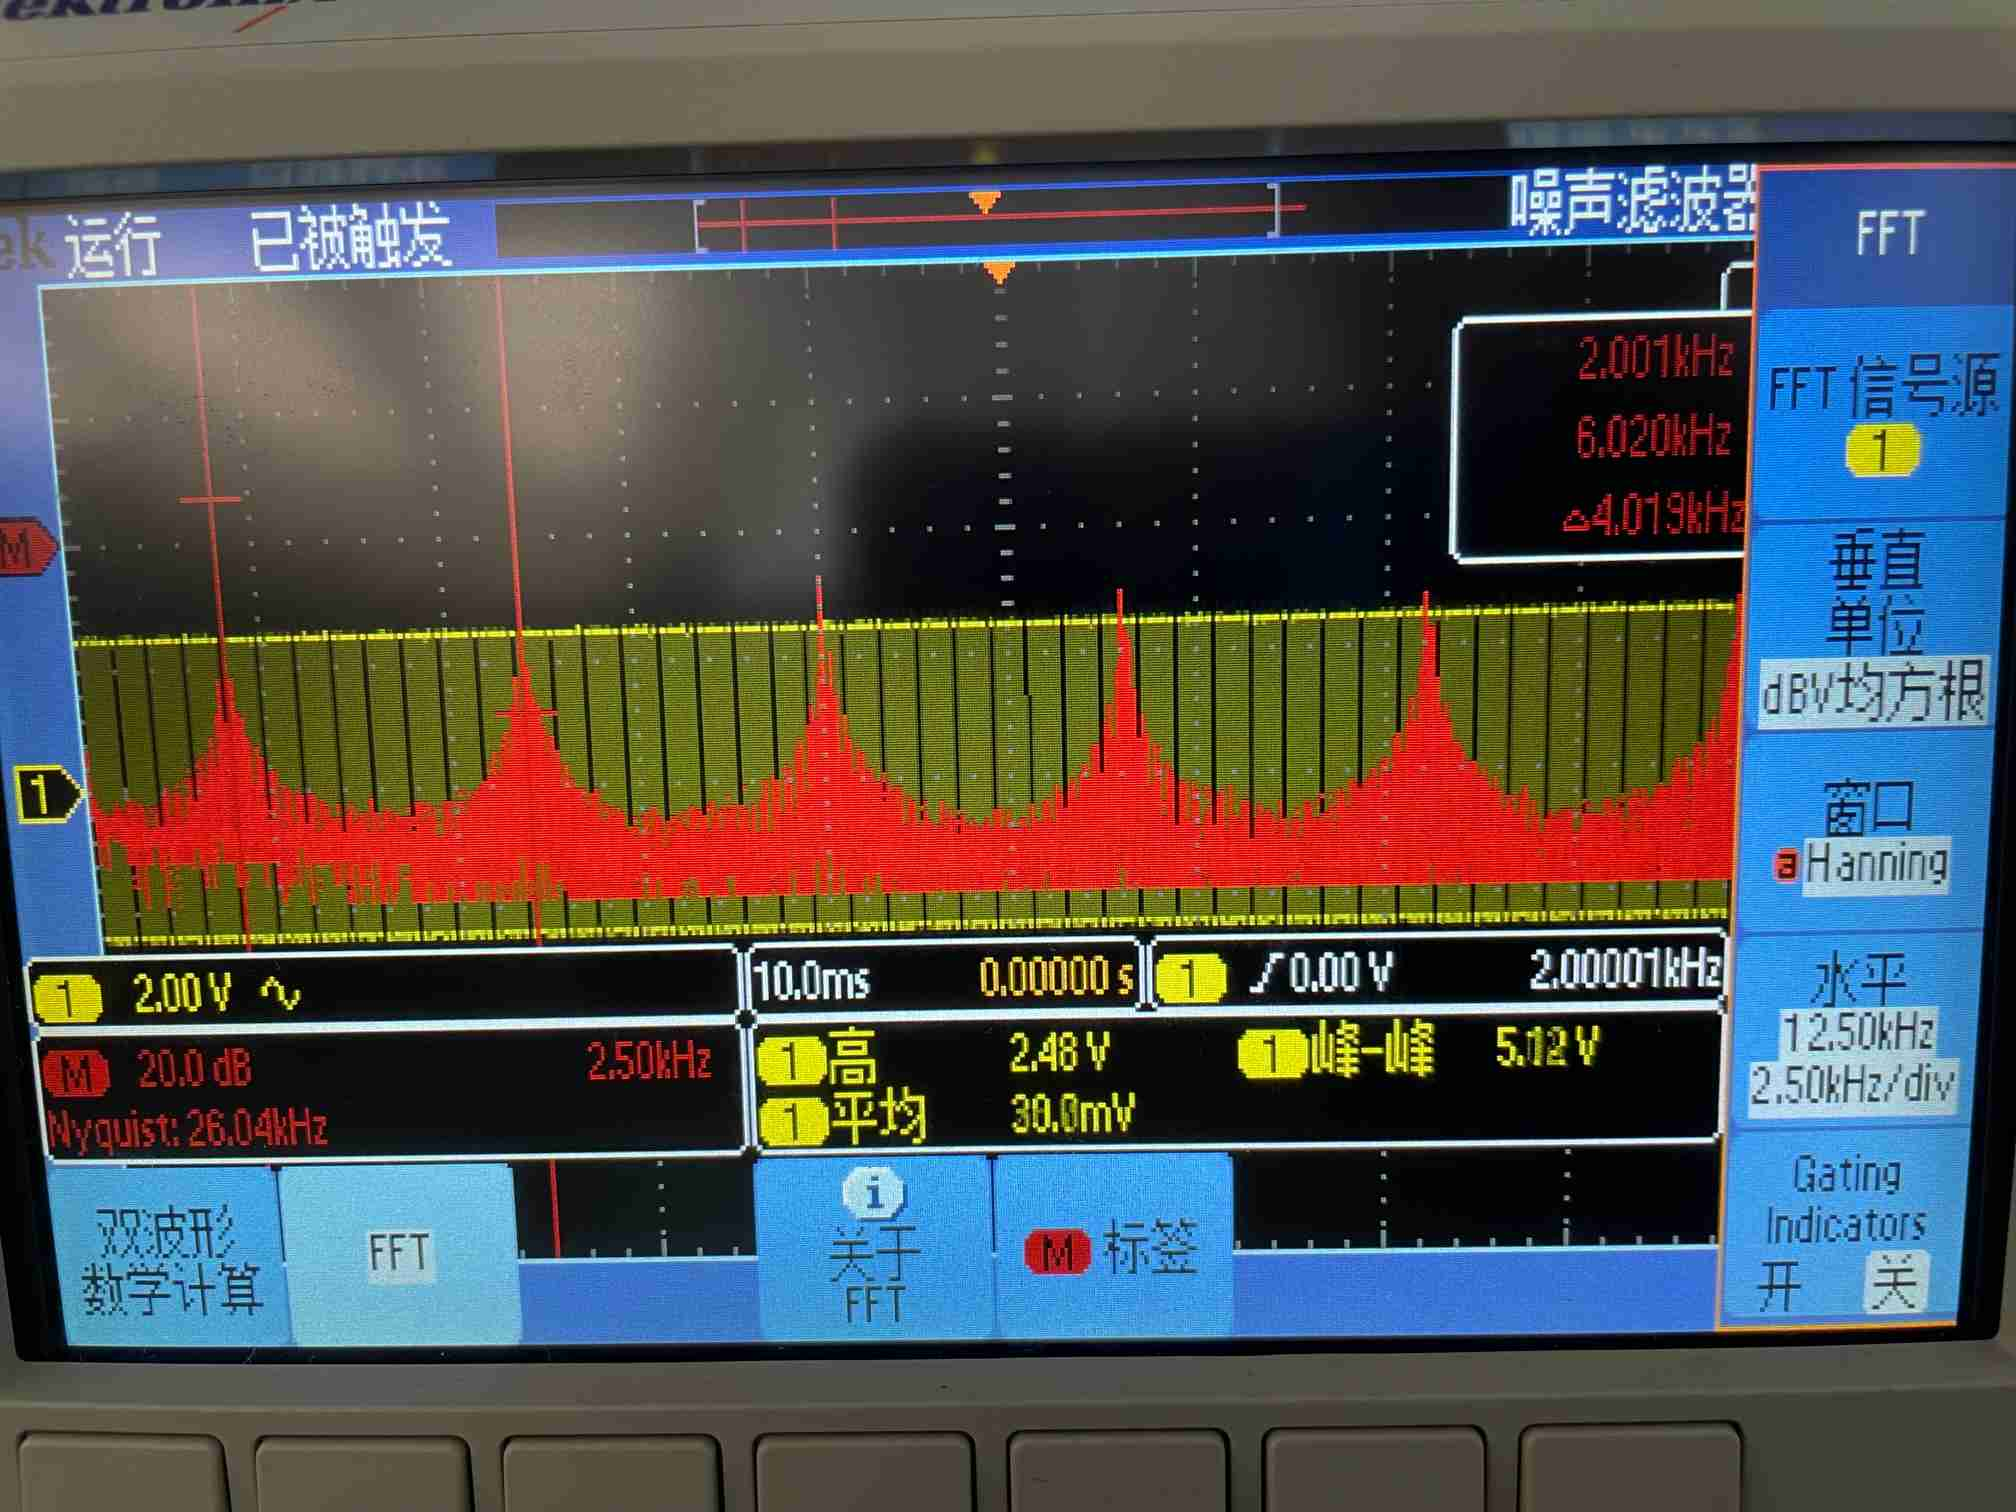
\includegraphics[width=0.3\textwidth]{hanning_squ_osc.jpg}
    }
    \caption{示波器测量方波信号时频域波形}
  \label{示波器2a(2)}
\end{figure}

如图\ref{示波器2a(2)}各子图示波器界面右上角所示,左侧光标Cursor在频率约2kHz处,右侧光标Cursor在频率约6kHz处,可知2kHz周期方波的频谱相邻两峰间隔约4.0kHz。

\subsubsection{示波器测量方波信号结果分析}
观察图\ref{示波器2a(2)}波形,相对另外三种窗函数,矩形窗窗函数的测量有较明显的混叠现象,这是由于矩形窗的频谱泄漏最为严重,进而在周期方波的多个周期性频点之间产生混叠;Blackman-Harris、汉明、汉宁窗的频谱泄漏程度相对较小,因此在频点较接近的周期信号的测量中,更适合用后者而不宜采用矩形窗。

四种窗函数下形成的频谱均能良好地观察到方波信号的各个频点,这是由于测量过程中采用了足够小的频率分辨率$\Delta f$。由前述,示波器分辨率带宽 = 1 /(时基长度$\times$水平格子数),测量方波过程中,调节时域水平旋钮,尽可能增加时基,从而减小频率分辨率。当频率分辨率$\Delta f<4k Hz$时,即能区分2000Hz方波的相邻频点峰值。
\subsubsection{M2K测量方波信号}
\textbf{实验要求b}:用M2K产生一个 2KHz 的周期方波,并用M2K中
的示波器和频谱仪观测信号,重复a)中的实验项目。

\textbf{实验过程}:在SCOPY界面,点击Signal Generator,将波的类型设置为Rectangular,频率设为2kHz。点击运行按钮。

点击Spectrum Analyzer,调节扫频范围,使呈现约十个频点峰值。依次选择汉明窗、汉宁窗、矩形窗后,点击运行按钮,观察到频谱如下:

\begin{figure}[H]
    \centering
    
    \subfigure[subfigure 1-1][汉明窗频谱测量]{
        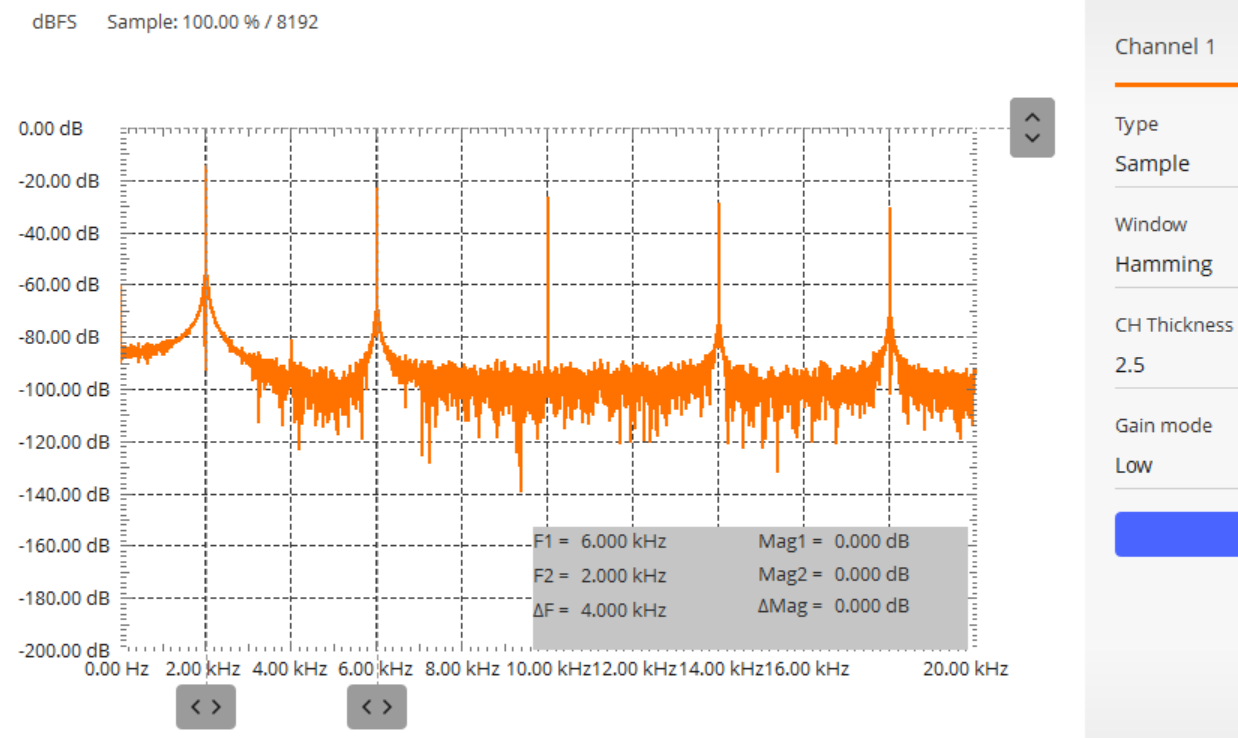
\includegraphics[width=0.3\textwidth]{scopy_squ_hamming.png}
    }
     \hspace{0.005\linewidth}
      \subfigure[subfigure 1-2][汉宁窗频谱测量]{
        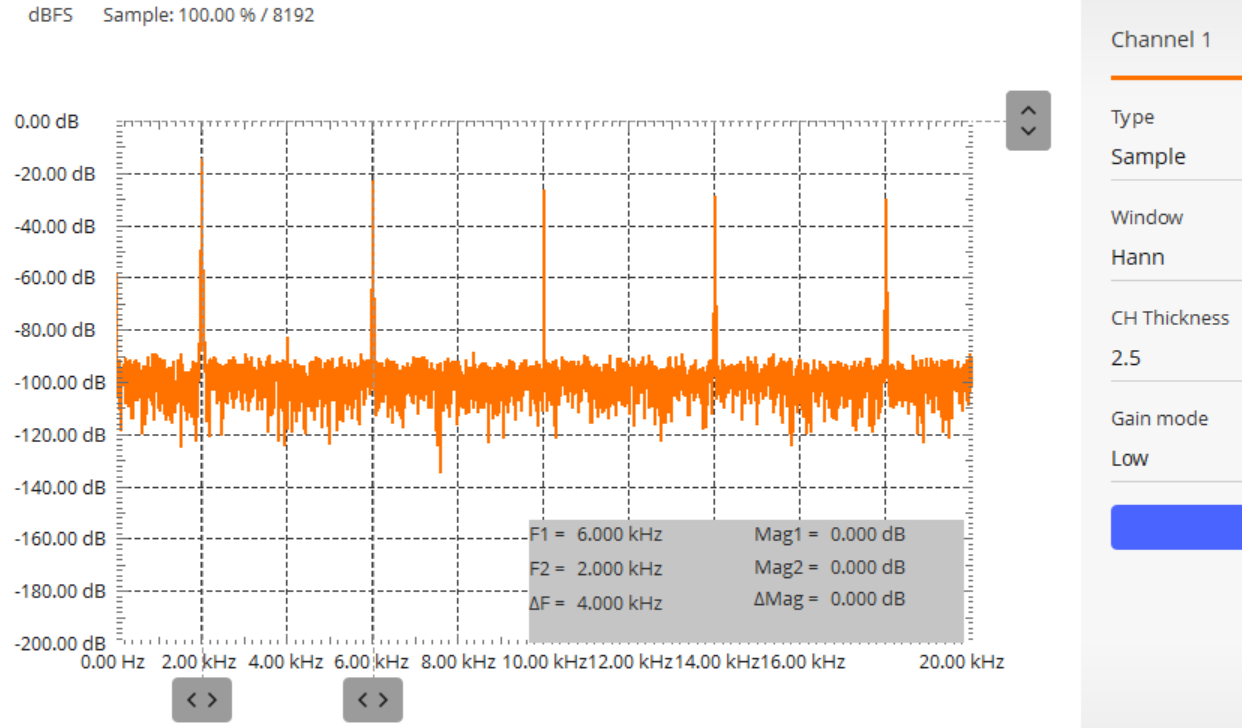
\includegraphics[width=0.3\textwidth]{scopy_squ_hann.png}
    }
         \hspace{0.005\linewidth}
      \subfigure[subfigure 1-3][矩形窗频谱]{
        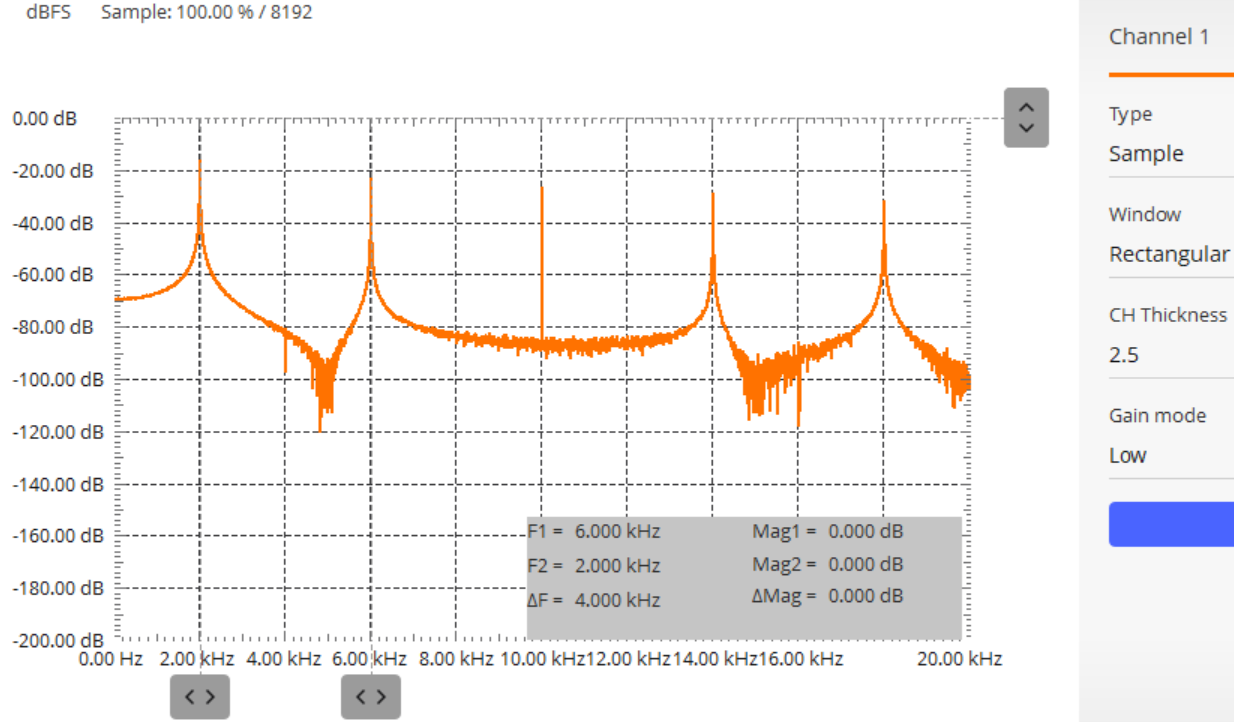
\includegraphics[width=0.3\textwidth]{scopy_squ_rect.png}
    }
    \caption{Scopy测量方波信号频域波形}
  \label{Scopy_square}
\end{figure}
Scopy测量结果如图\ref{Scopy_square}所示,测量
第一个峰值频点与第二个峰值频点,依次为2kHz及6kHz,相邻峰值频点间隔4kHz。

如子图6(b),汉宁窗的频谱能量集中程度最好,源于汉宁窗旁瓣衰减较大;如子图6(c),矩形窗的频谱泄漏最严重,源于矩形窗不对信号不连续点产生衰减。




\subsubsection{MATLAB编程实现方波信号幅度谱}

\textbf{实验要求c}:用MATLAB产生一个 2KHz 的周期方波,用不同宽
度的窗函数进行截断,通过编程绘制出其幅度谱,
并说明其与宽度变化的关系,并说明与a),b)中的
差别及其原因。

\textbf{实验过程}:傅里叶变换与实验一程序相近,将输入信号改为周期方波,采用square()函数实现,剩余代码不再赘述。
\begin{lstlisting}
    clear;clc;
    f = 2000;
    t1 = -0.001;t2 = 0.001; %t1 = -t2,分别选用窗长0.002,0.01及0.05观察频谱
    f1 = 0; f2 = 10000; df = 1;
    T = t2 - t1; dt = T / 20000;
    t = t1:dt:t2;
    x = square(2 * pi * f * t); 
\end{lstlisting}

MATLAB实验结果如下所示:
\begin{figure}[H]
    \centering
    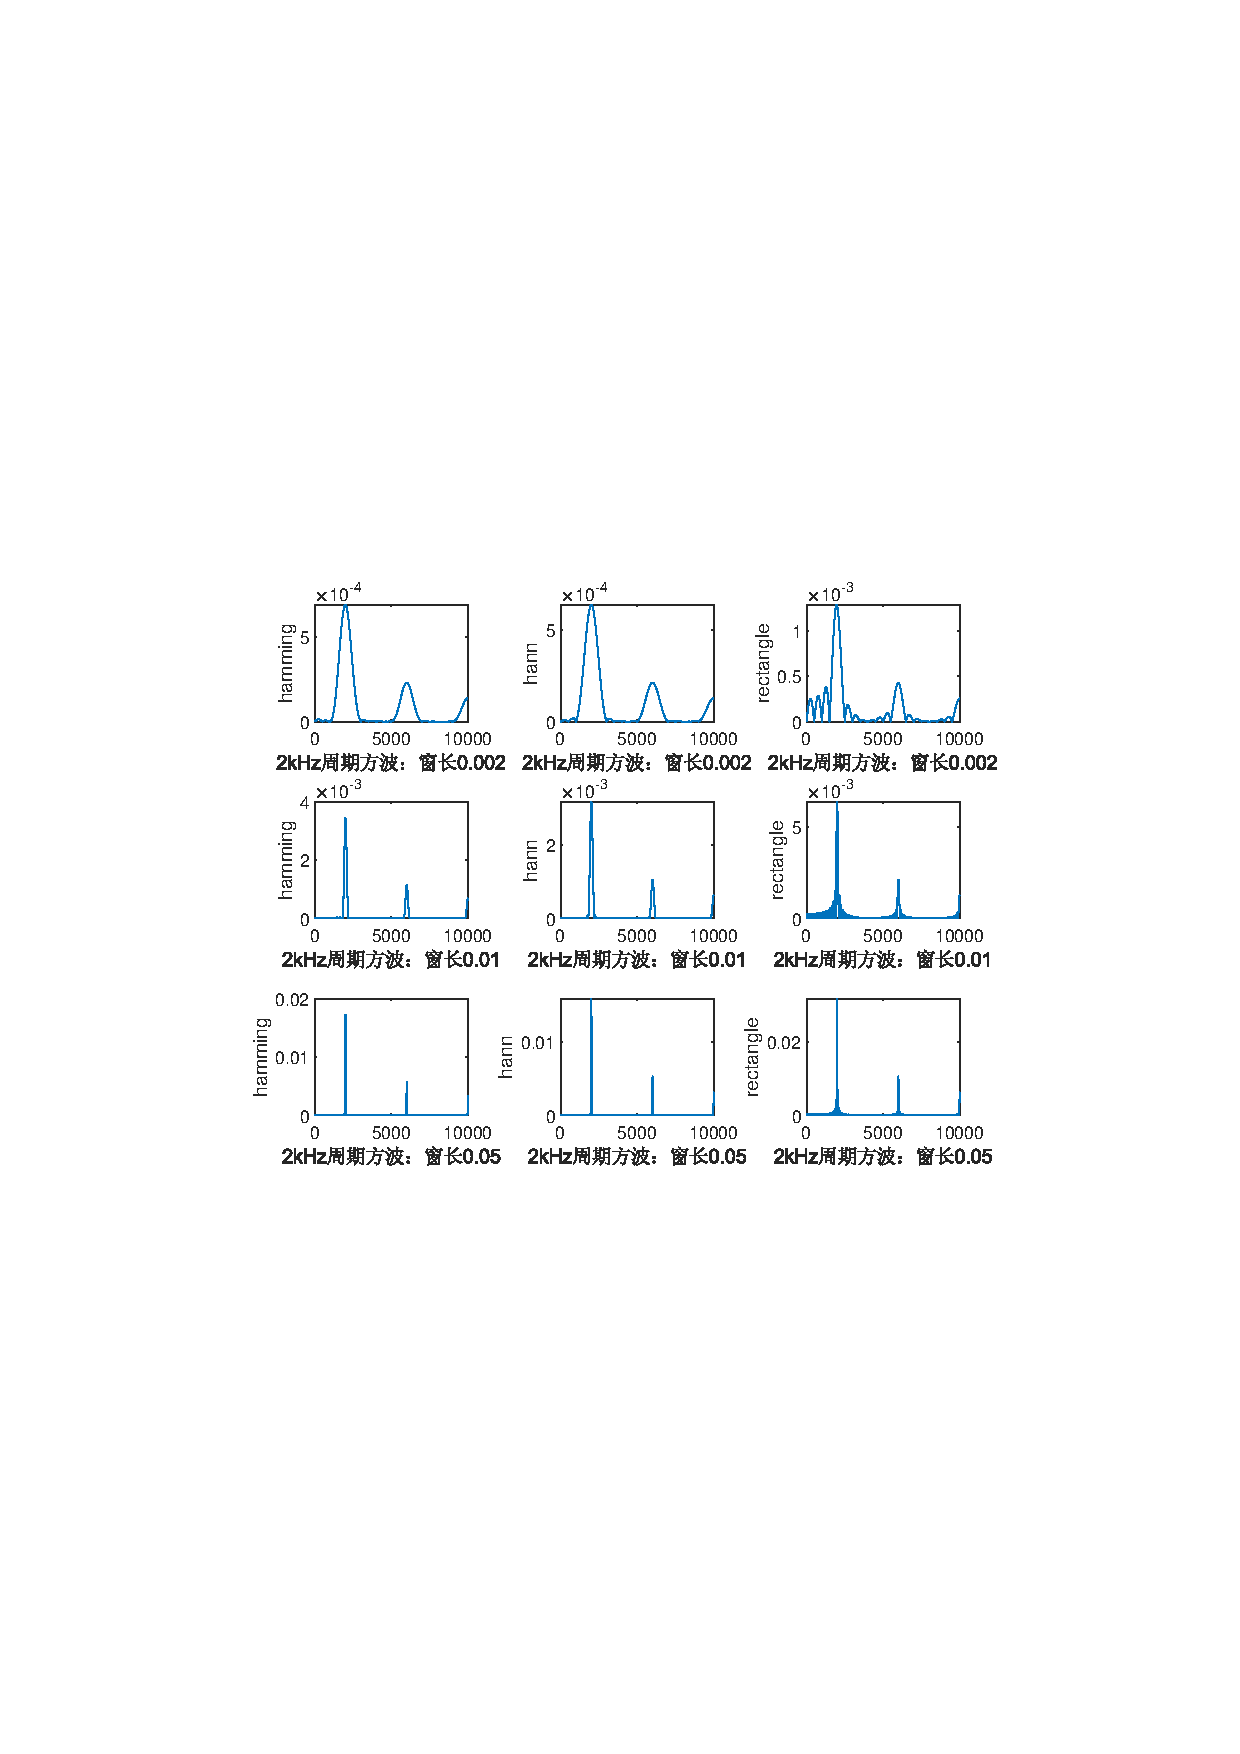
\includegraphics[scale=1]{matlab_squ.pdf}
    \caption{MATLAB加窗绘制周期方波信号(2kHz)频谱}
    \label{matlab_square}
\end{figure}

\subsubsection{窗函数宽度与方波信号幅度谱的关系}
如图\ref{matlab_square},纵向对比同种窗函数下幅度谱的变化,随着窗的宽度增加,每个频点的能量逐渐集中,且频谱泄漏程度减小。这是由于方波可看作是一系列单音信号的叠加,因此在各频点上的变化趋势与单音信号是一致的。同样满足如式\ref{omega}的推导。

同时,窗函数宽度增加,单个频点幅度谱的幅值升高,对应该频点能量更集中。

\subsubsection{MATLAB仿真与示波器、Scopy测量方波的对比分析}
\begin{itemize}
    \item 产生信号的差异:MATLAB仿真信号不产生毛刺,而示波器和M2K信号中含大量毛刺,这基于物理信号源的测量需考虑仪器底噪和环境白噪声。
    \item 频谱产生方式的差异:MATLAB仿真生成方波频谱时,主要考虑采样点是否足够,窗函数宽度是否足够等问题,只要采样点N、窗长T足够大,即可仿真得到近似的方波频谱;而示波器测量需要考虑频谱分辨率是否足够小,只有频谱分辨率小于4kHz,才能区分相邻两个频点,并使非频点处幅值衰减。
    \item 幅值的差异:MATLAB仿真模拟形成的方波幅度谱,从2kHz开始,每增加4kHz,对应频点处尖峰幅值下降,依次衰减;而示波器与M2K各频点处幅度不产生衰减。这基于MATLAB采用傅里叶变换得到方波频谱,而示波器、M2K采用FFT变换,幅值不受影响。
\end{itemize}



\subsection{实验三(选做):信号卷积}
\textbf{实验要求}:已知某系统单位冲激响应为$h(t)=1,0\le t\le1$,用一个从$t=1$开始,宽度为1,幅度为1的矩形脉冲$x(t)$激励系统,得到输出信号:
\begin{itemize}
\setlength{\itemsep}{0pt}
\setlength{\parsep}{0pt}
\setlength{\parskip}{0pt}
    \item 通过MATLAB编程画出$x(t),h(t),y(t)$的波形;
    \item 将$h(t),y(t)$用SCOPY波形发生功能显示出来;
    \item 将$y(t)$再次通过这一系统,重复上述任务;
    \item 在MATLAB中用相关函数(xcorr)实现任务1,并解释相关和卷积的区别。
\end{itemize}

\textbf{实验过程}:(a)编写代码,构造$x(t)$与$h(t)$,并用卷积函数conv()求得$y(t)$,代码如下:
\begin{lstlisting}
    dt = 0.01; t = -1:dt:4; %时域步长dt设置为0.01
    h = ((t > 0) - (t > 1)); % 以MATLAB语法(t > t0)实现阶跃函数u(t - t0),其中用到bool计算结果
    x = ((t > 1) - (t > 2));
    ty = linspace(2 * t(1),2 * t(end),2 * length(t) - 1); % y的卷积结果在时域上是x(t)及h(t)时间轴的最小值之和至两者时间轴的最大值之和,且y的精度相比x与h,不发生改变
    y = conv(x,h) * dt; %conv默认卷积步长是1,因此幅值需乘以时域步长
    
    subplot(1,3,1); plot(t,x);
    xlabel('t'); ylabel('x(t)');
    subplot(1,3,2); plot(t,h);
    xlabel('t'); ylabel('h(t)');
    subplot(1,3,3); plot(ty,y);
    axis([-1 4 0 1])
    xlabel('t'); ylabel('y(t) = x(t) * h(t)');
\end{lstlisting}
程序运行结果如下所示:
\begin{figure}[H]
    \centering
    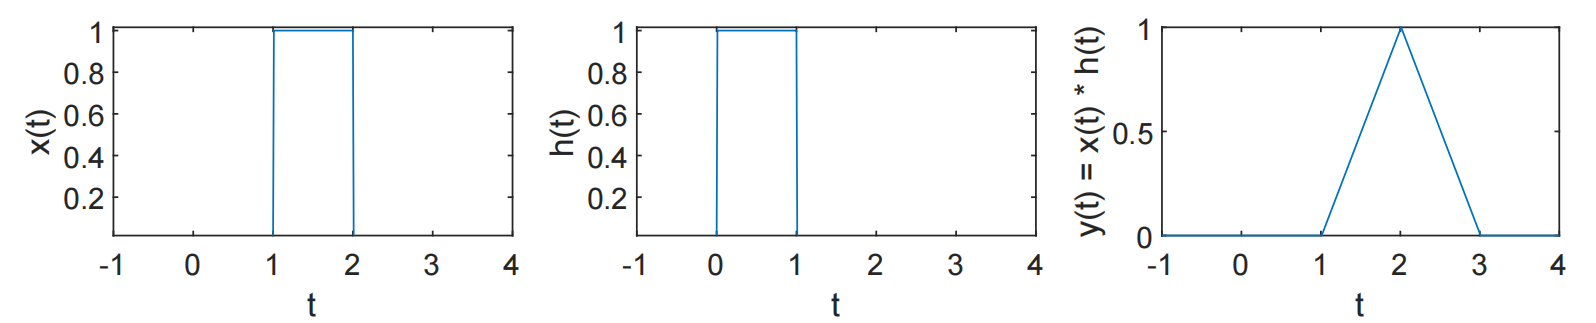
\includegraphics[scale=0.27]{conv1.png}
    \caption{卷积运算$y(t) = x(t) * h(t)$}
    \label{conv_a}
\end{figure}

(b)将$h(t)$和$y(t)$用Scopy的波形发生功能显示出来。

将MATLAB 中$h(t),y(t)$幅值点以列向量形式存入csv文件,如下所示:
\begin{lstlisting}
    writematrix(h', 'h(t).csv')
    writematrix(y', 'y(t).csv')
\end{lstlisting}
选中Scopy中Signal Generator,并在Buffer中导入csv文件,得到波形如下:
\begin{figure}[H]
    \centering
    
    \subfigure[subfigure 1-1][$h(t)$信号]{
        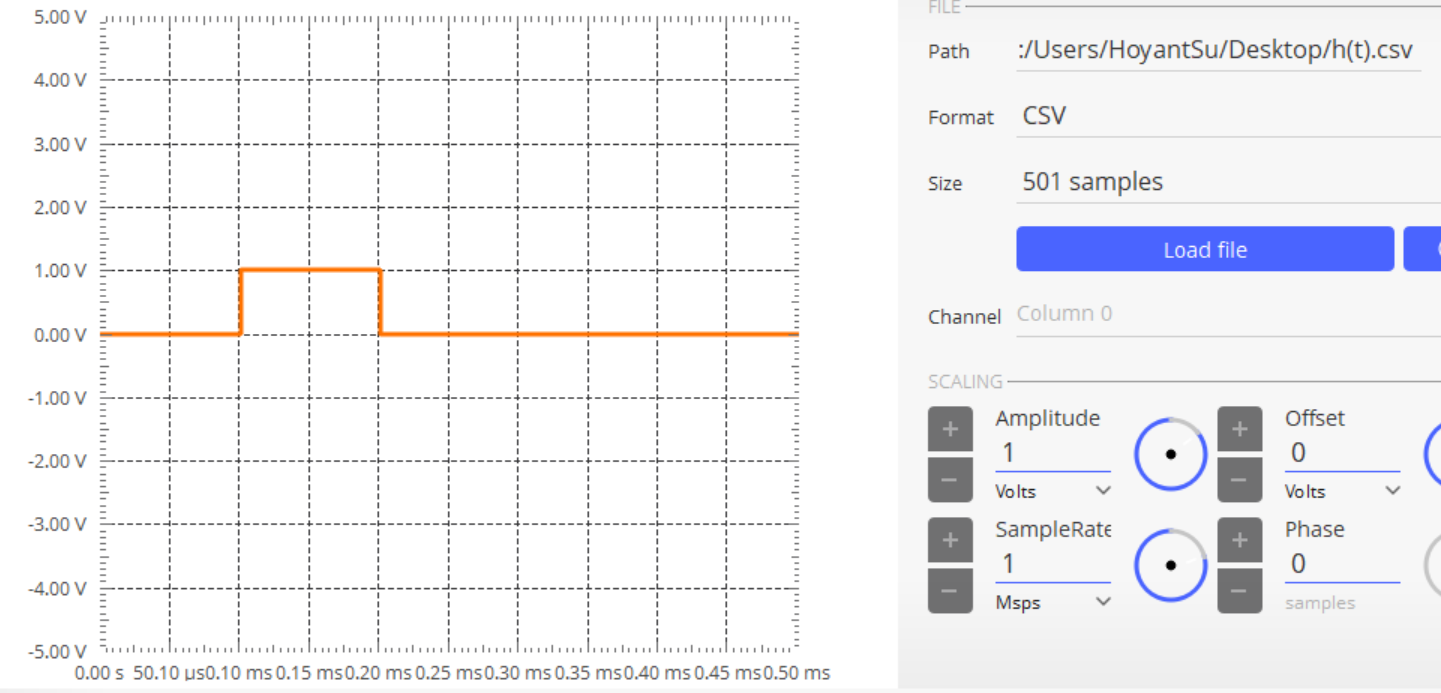
\includegraphics[width=0.35\textwidth]{experiment3_1.png}
    }
     \hspace{0.005\linewidth}
      \subfigure[subfigure 1-2][$y(t)$信号]{
        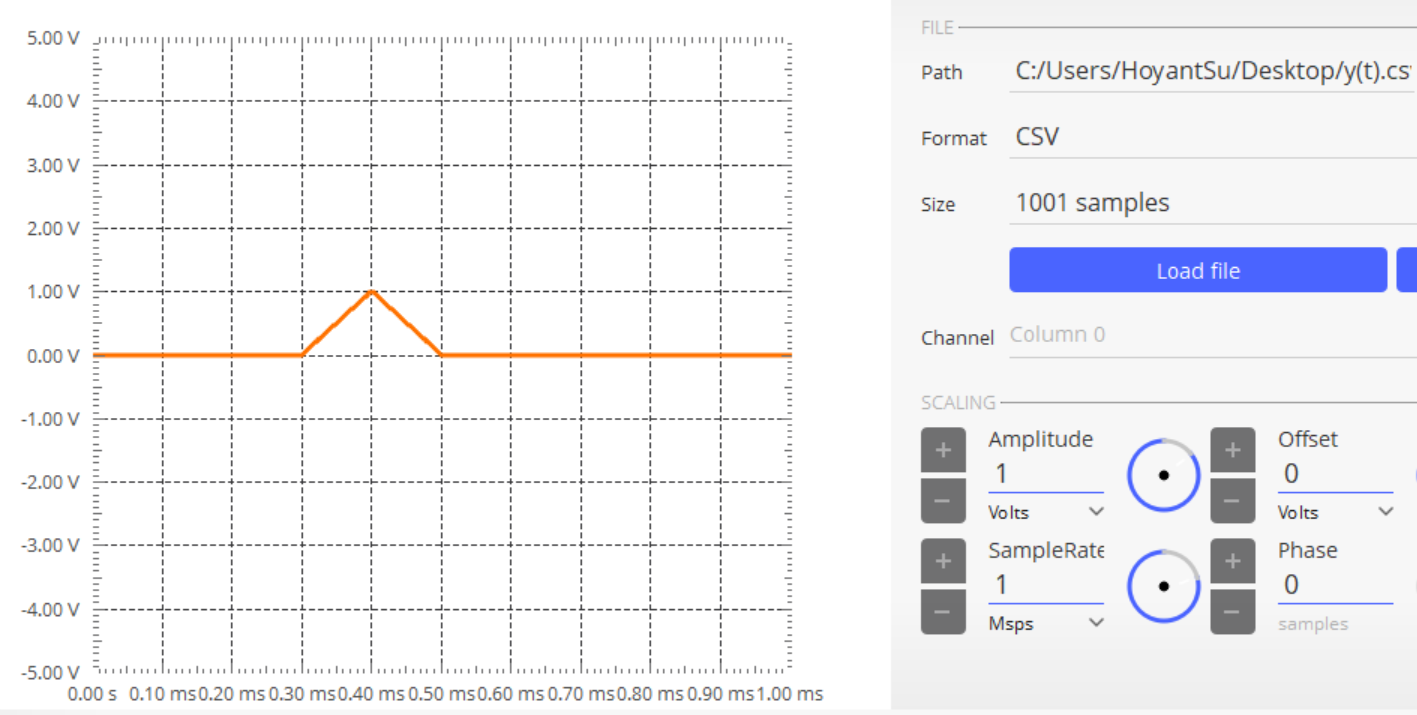
\includegraphics[width=0.35\textwidth]{experiment_3_2.png}
    }
       
    \caption{Scopy显示信号时域仿真波形$h(t),y(t)$}
  \label{示波器2a(2)}
\end{figure}

(c)编写代码,令$y(t)$再次通过系统,假定得到输出$y_2(t)=y(t) * h(t)$。
\begin{lstlisting}
    %%%%%%%%%延续之前的代码部分%%%%%%%%%%%
    ty2 = linspace(t(1) + ty(1),t(end) + ty(end),length(ty) + length(t) - 1);
    y2 = conv(y,h) * dt;
    subplot(3,1,1); plot(t,h); axis([-1 4 0 1]);
    xlabel('t'); ylabel('h(t)');
    subplot(3,1,2); plot(ty,y); axis([-1 4 0 1]);
    xlabel('t'); ylabel('y(t)');
    subplot(3,1,3); plot(ty2,y2); axis([-1 4 0 1]);
    xlabel('t'); ylabel('y2(t)');
\end{lstlisting}
程序运行结果如下所示:
\begin{figure}[H]
    \centering
    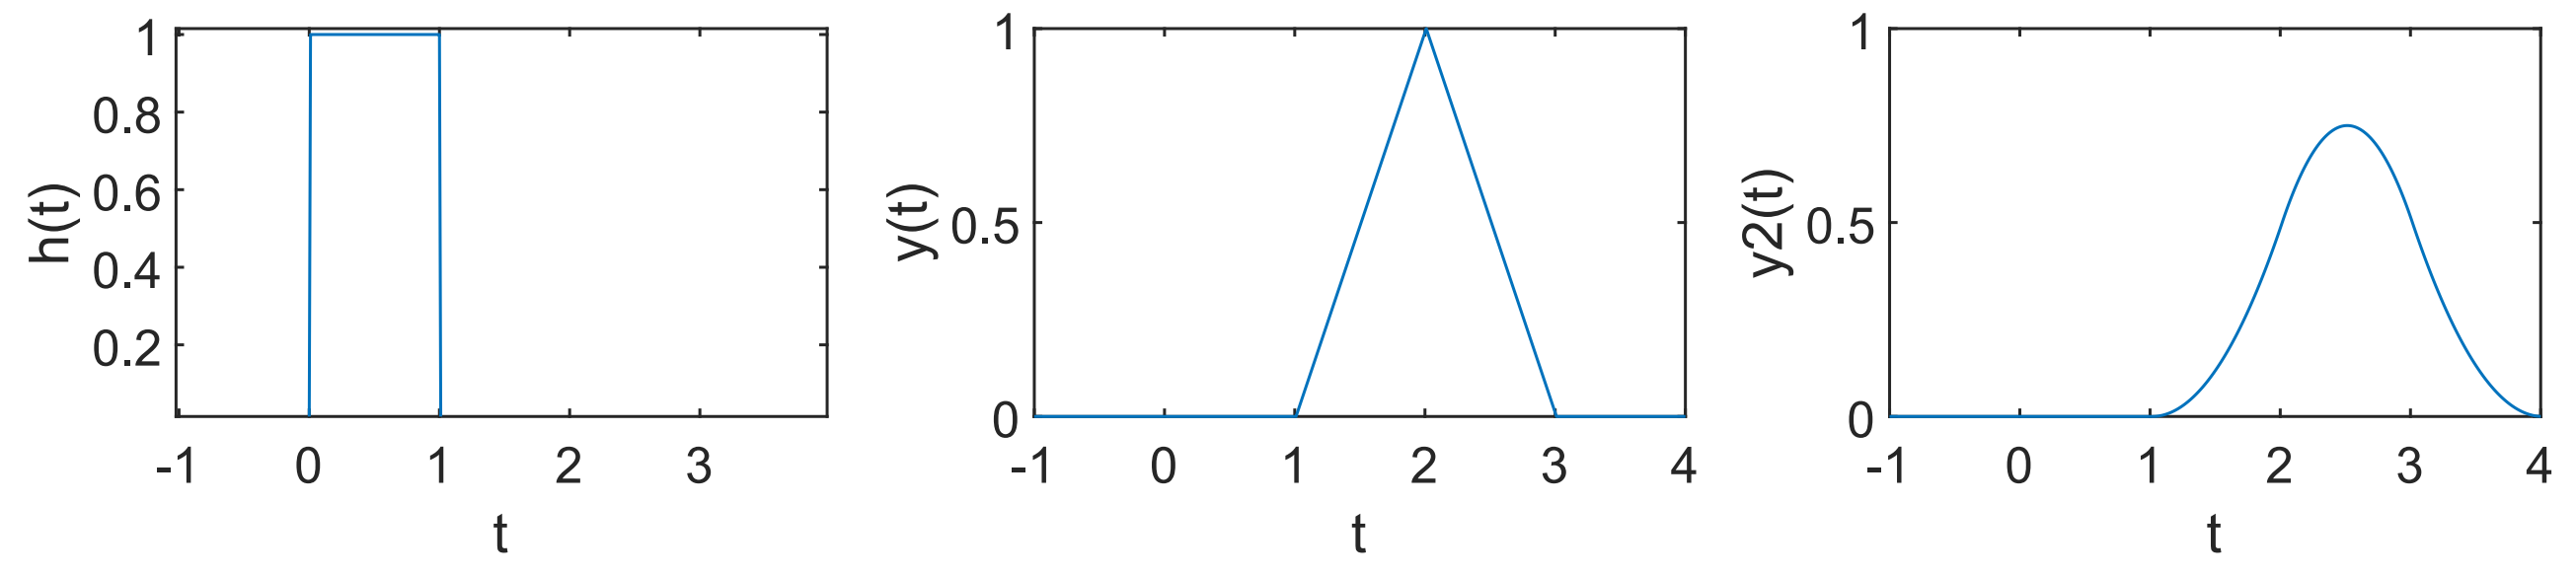
\includegraphics[scale=0.16]{conv3.png}
    \caption{卷积运算$y_2(t)=y(t)*h(t)$}
    \label{conv_c}
\end{figure}

用Scopy显示$h(t)$及$y_2(t)$波形,如下所示:
\begin{figure}[H]
    \centering
    
    \subfigure[subfigure 1-1][$h(t)$信号]{
        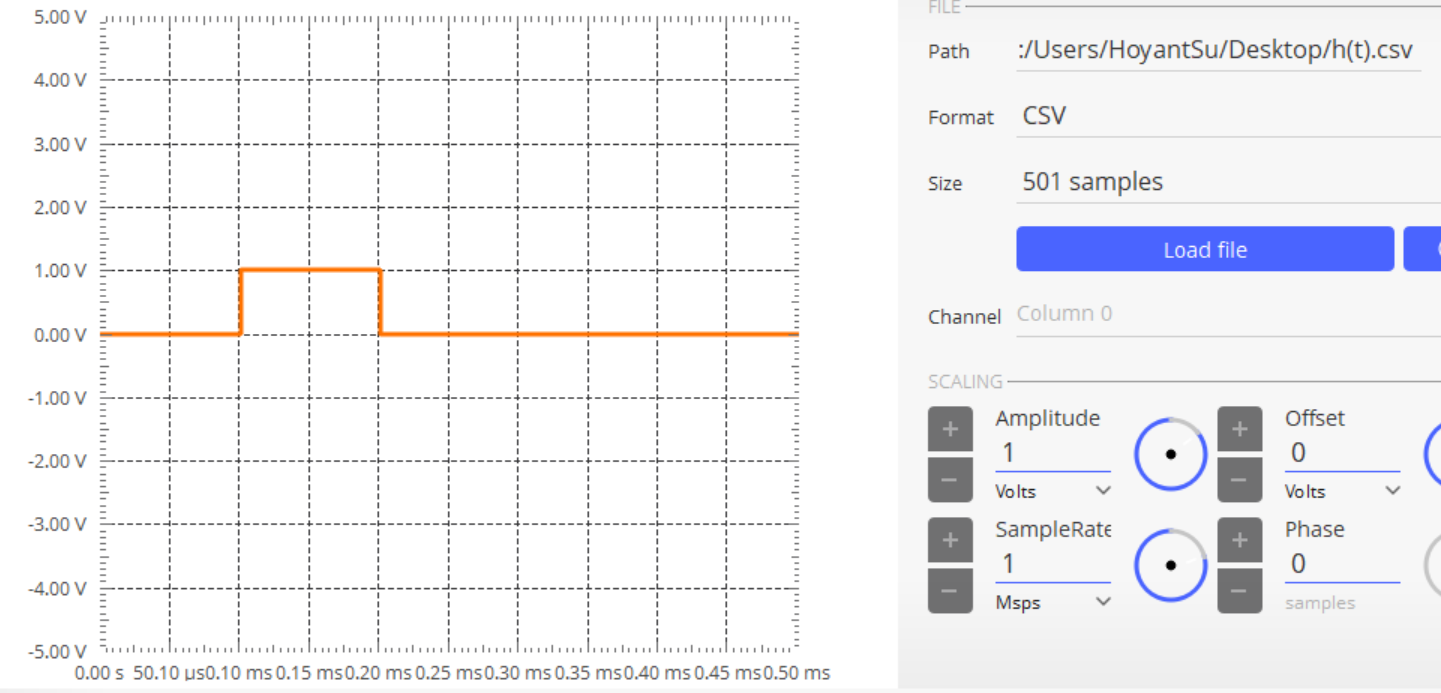
\includegraphics[width=0.35\textwidth]{experiment3_1.png}
    }
     \hspace{0.005\linewidth}
      \subfigure[subfigure 1-2][$y(t)$信号]{
        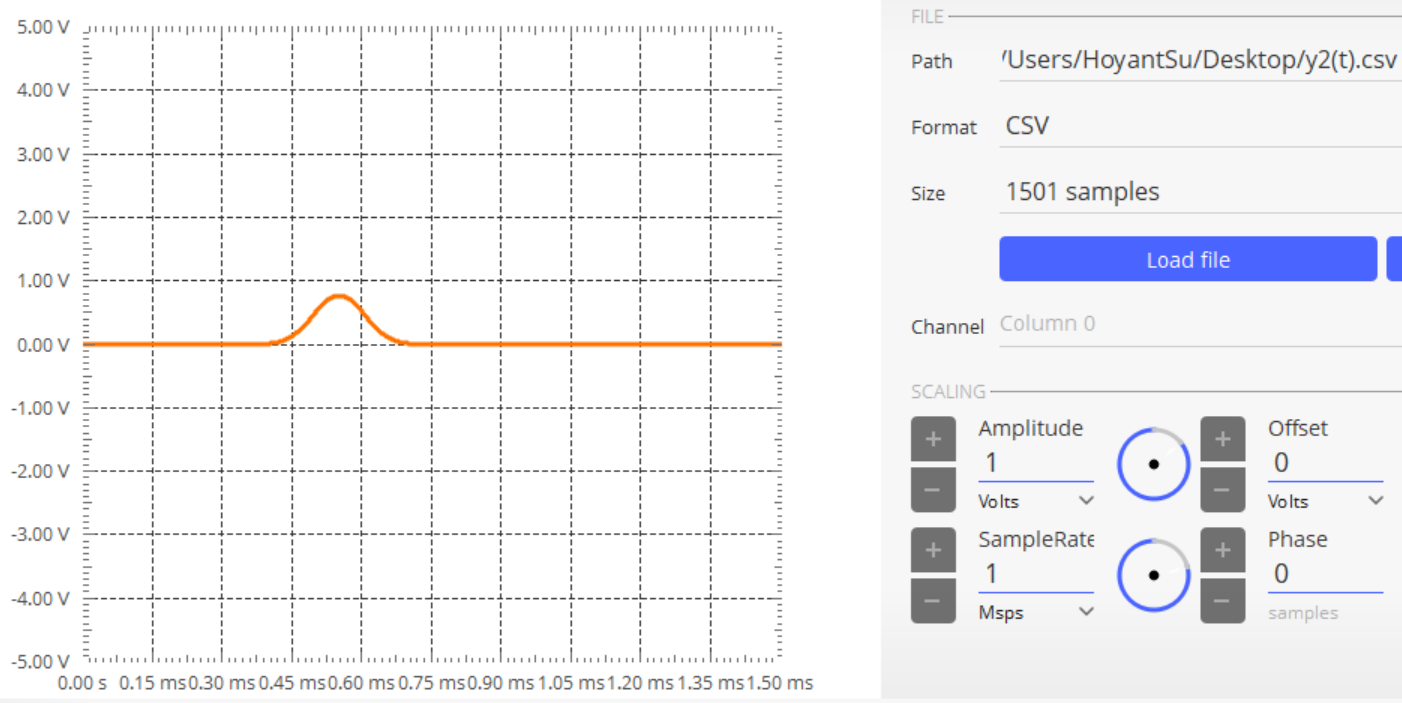
\includegraphics[width=0.35\textwidth]{experiment3_3.png}
    }
    \caption{Scopy显示信号时域仿真波形$h(t),y_2(t)$}
  \label{示波器2a(2)}
\end{figure}


(d):将卷积运算$y(t)=x(t) * h(t)$改用相关函数xcorr()实现,编程如下:
\begin{lstlisting}
dt = 0.01;
t = -1:dt:4;
h = ((t > 0) - (t > 1));
th = -t(end:-1:1); %时域t沿y翻折得到th:范围-4-1
h2 = ((th > -1) - (th > 0)); %h(t)沿y翻折得到h2(t)
x = ((t > 1) - (t > 2));
ty = linspace(-th(end) + t(1),t(end) - th(1),length(th) + length(t) - 1);  %做相关运算对应相关函数的定义域范围
y = xcorr(x,h2) * dt;
subplot(3,1,1); plot(t,x);
xlabel('t'); ylabel('x(t)'); axis([-1 4 0 1]);
subplot(3,1,2); plot(t,h);
xlabel('t'); ylabel('h(t)'); axis([-1 4 0 1]);
subplot(3,1,3); plot(ty,y); axis([-1 4 0 1]);
xlabel('t'); ylabel('$y(t) = \int x(t)\cdot h^*(t-\tau)\mathrm{d}t$','interpreter','latex'); %相关运算
\end{lstlisting}
代码运行结果与图\ref{conv_a}相一致。其中,绘制$h_2(t)$时域图,恰好为$h(t)$沿y轴的翻折。
\\\hspace{\zfill}\\
\textbf{卷积与相关的区别:}
\begin{itemize}
\item 从定义上:对两个信号$f_1(t)$和$f_2(t)$,卷积$f_c(t)$定义为:$f_c(t)=\int_{\mathbb{R}}f_1(\tau)f_2(t-\tau)\mathrm{d}\tau$。相关$R_{12}(\tau)$定义为$R_{12}(\tau)=\int_{\mathbb{R}}f_1(t)f_2^*(t-\tau)\mathrm{d}t$。
\item 从形式上:两个信号卷积可看作一个信号先沿y轴翻折,再在时域轴上平移求积分的过程;两个信号的相关没有经过翻折,表现为两个复函数的共轭内积。
    \item 物理意义:卷积可看作是在时刻对系统进行观察,输出为过去产生的所有信号经过系统的处理/响应后得到的结果的叠加,是加权求和的过程;相关可看作是一个函数对另一个函数在时域上的扫描,运算结果反映出两者的相似程度。
\end{itemize}


\section{实验讨论}
\subsection{信号频域分析加窗的原因讨论}
从数学角度,周期信号的傅里叶变换不存在,因为其不满足绝对可积的条件。但对周期信号做截断处理,将时域限制在有限范围内,再延拓到全域,可以认为傅里叶变换是存在的。从而可使用MATLAB对周期信号做傅里叶变换。

从FFT变换原理角度,FFT算法将采样的信号认为是无限长的周期的信号,其在时域和频域上形成环形拓扑结构。但实际采样中所得信号由有限个采样点构成,在FFT运算后有限个点重复排列构成环形,这样就有可能出现波形突然不连续的情况,进而导致频谱泄漏。
加窗可以使不连续的位置更平滑,从而消除这种突变。


\subsection{信号截断产生频谱泄漏的原因讨论}
窗函数在时域上往往上有限的,因此其是频带无限的函数。窗函数在时域上对原信号截断后,在频域上与信号卷积,从而使输出信号含无限带宽,即信号再频域的能量与分布被扩展。

由采样定理,输出信号在频域上搬移,由于输出信号带宽无限,所以一定产生混叠。





\subsection{周期方波频谱的推导}
实验中观察到,当采样点足够多时,周期方波偶次频点的幅值应无限接近0。可采用周期信号傅里叶变换的思想及傅里叶级数的思想解释。
\subsubsection{以周期函数傅里叶变换思想推导周期方波频谱}
由周期函数$f_T(t)$傅里叶变换,若其有限单位周期函数为$f(t)$及其傅里叶变换为$F(\omega)$,则有
\begin{center}
    {\setlength\abovedisplayskip{-0.8cm}
    \setlength\belowdisplayskip{-0.2cm}
    \begin{equation}
        \begin{aligned}
            f_T(t)\longleftrightarrow \omega_0 \sum_{k=-\infty}^{\infty}F(k\omega_0)\delta(\omega-k\omega_0)\\
        \end{aligned}
    \end{equation}
    }
\label{Fourier_periodic}
\end{center}

以MATLAB生成的square()函数为例,其有限单位周期函数$f(t)$满足:
\begin{center}
        {\setlength\abovedisplayskip{-0.5cm}
        
    \begin{equation}
 f(t)=   
\left\{\begin{matrix}
 1 & 0<t\le\frac{T}{2}\\
-1   & \frac{-T}{2}<t\le 0
\end{matrix}\right.
    \end{equation}
    }
\end{center}
则
\begin{center}
        {\setlength\abovedisplayskip{-0.8cm}
       
        \begin{equation}
            \begin{aligned}
                    f(t)\longleftrightarrow F(\omega)&=\int_{-\infty}^{\infty}f(t)\mathrm{e}^{-\mathrm{j}\omega t}\mathrm{d}t\\
                    &=\int_{-T/2}^{0}f(t)\mathrm{e}^{-\mathrm{j}\omega t}\mathrm{d}t+\int_{0}^{T/2}f(t)\mathrm{e}^{-\mathrm{j}\omega t}\mathrm{d}t\\
                    &=\frac{2}{\mathrm{j}\omega}\cdot(1-\mathrm{e}^{-\mathrm{j}\omega \frac{T}{2}})\\
                \stackrel{\ref{Fourier_periodic}}\Longrightarrow F_T(\omega)&= \omega_0 \sum_{k} \frac{2}{\mathrm{j}k\omega_0}\cdot(1-\mathrm{e}^{-\mathrm{j}k\omega_0 \frac{T}{2}})\cdot\delta(\omega-k\omega_0) \\  
                 \stackrel{\omega_0\cdot T=2\pi}\Longrightarrow |F_T(\omega)|&=\sum_k \frac{2}{k}\cdot|1-\mathrm{e}^{-\mathrm{j}k\omega_0 \frac{T}{2}}|\cdot |\delta(\omega-k\omega_0)|\\
                    &=\sum_k \frac{4}{k}|\sin 
                    \frac{k\pi}{2}|\cdot \delta(\omega-k\omega_0)\\
            \end{aligned}
        \end{equation}
        }
        \label{equ_fourier}
\end{center}
从而,当$k$为偶数时,周期方波的频谱分量为0;当$k$为奇数时,频谱幅度遵循$\frac{4}{k}\cdot \delta(\omega-k\omega_0)$。即高次信号的幅值与次数成反比关系。

\subsubsection{以傅里叶级数思想推导周期方波频谱}
由于傅里叶级数是傅里叶变换的极限形式,因此也可直接推导其离散频谱,解释$k$为偶数时,频谱分量为0的现象。
由离散频谱$\{C_k\}$表达式,
\begin{center}
           {\setlength\abovedisplayskip{-0.4cm}
           \begin{equation}
               \begin{aligned}
                C_k = &\frac{1}{T}\int_T f(t) \mathrm{e}^{-\mathrm{j}k\omega_0t}\mathrm{d}t\\
                = & \frac{1}{T}(\int_{-T/2}^0f(t)\mathrm{e}^{-\mathrm{j}k\omega_0t}\mathrm{d}t + \int_{0}^{T/2}f(t)\mathrm{e}^{-\mathrm{j}k\omega_0t}\mathrm{d}t)\\
                =&\frac{1}{T}\cdot \frac{2}{\mathrm{j}k\omega_0}\cdot(1-\mathrm{e}^{-\mathrm{j}k\omega_0 \frac{T}{2}})\\
                =&\frac{1}{T}\cdot \frac{2}{\mathrm{j}k\omega_0}\cdot (1-(-1)^k)\\
                 \Rightarrow |C_k|=&|\frac{1}{k\pi}(1-(-1)^k)|\\        
               \end{aligned}
           \end{equation}
           }
           \label{equ_fourier2}
\end{center}
从而解释了k为偶数时,幅度为0。

\subsubsection{采样点不足时,MATLAB模拟的周期方波产生其它频谱分量的原因讨论}
当采样点不足时,方波的频谱不仅在偶次频点上有较高的幅值出现,在其它频点上也出现了一定的幅值。一种可能的原因是由于采样点过少,未完全采样时域信号,即实际采集到的信号不为矩形,可能为梯形信号,从而导致傅里叶变换后,没有表现出方波信号的频谱形状。



\section{实验总结}
本次实验通过示波器、M2K测量单音信号及方波信号,从实践层面理解了FFT工作原理、信号加窗原理;通过MATLAB编程,掌握了工程软件实现傅里叶变换方法、时频域变换原理、卷积与相关的关系、窗函数宽度与频谱的关系,体会到MATLAB矩阵乘法的优越性。

在预习实验“傅里叶变换的数值计算”中,掌握了双重循环及向量/矩阵乘法实现傅里叶变换,由表\ref{runtime},推导得出双重循环法时间复杂度更大,为$O(n^2)$,而向量/矩阵乘法则借助MATLAB高性能数学库,运算处理时间更短。

在实验一“单音2kHz正弦波测量”中,掌握了采用示波器FFT测量单音信号方法,由图\ref{示波器1a}、\ref{示波器1a(2)}、\ref{Scopy_sine},对比得出矩形窗的高频率分辨能力,而汉宁/汉明窗的频谱泄漏消除能力较强。由图\ref{MATLAB_sin},得出窗函数宽度增加有助于中心频率的集中,减小频谱的泄漏程度。从四个角度:产生信号、频点、频率分辨率、幅度,具体分析了三种测量方法的差异。

在实验二“2kHz方波测量”中,掌握了采用示波器FFT测量方波信号方法,并推导得出示波器分辨率带宽与时基的倒数关系,掌握了调整时基以抬高频谱分辨率的方法。由图\ref{示波器2a(2)}、\ref{Scopy_square},得出在频点接近的周期信号测量中,宜使用使频谱泄漏程度较小的窗函数,如汉宁/汉明/Blackman-Harris。由图\ref{matlab_square},得出窗函数宽度增加有助于方波频谱能量集中的结论。从三个角度:产生信号、频谱产生方式、幅值,具体分析了三种测量方法的差异。

在实验三“信号卷积”中,掌握了MATLAB计算卷积及相关的方法,学会了conv()及xcorr()函数的使用,对信号定义域的范围确定有了更深的理解,得到卷积结果如图\ref{conv_a}、\ref{conv_c}所示。从三个角度:定义、形式、物理意义上,系统分析了卷积与相关的区别。

在实验讨论中,从数学及FFT变换原理角度探讨了信号加窗的原因;从窗函数性质与采样定理角度探讨了信号截断产生频谱泄漏的原因;从周期函数傅里叶变换及傅里叶级数角度推导得出周期方波偶次频点为0的原因,如式\ref{equ_fourier}、\ref{equ_fourier2}所示。分析了采样点不足时,MATLAB模拟周期方波出现其它频谱分量的原因。

本次实验启发了我对实际FFT测量中合理选择窗函数的思考,认识到傅里叶变换的工程实现是复杂的,这些在理论推导中是无法得出的。通过本次信号时频域分析实验,让我对模拟信号的数字化处理过程有了新的认识,收获颇丰。感谢在实验中多次指导帮助我的老师和助教!











\end{document}
